%\VignetteEngine{knitr::knitr}
%\VignetteIndexEntry{Starting with bipartite}
%\VignetteEncoding{UTF-8}

\documentclass[a4paper, 11pt]{article}
%\usepackage[sc]{mathpazo}
%\usepackage{authblk} % authors & affiliations
\usepackage[utf8]{inputenc}
\usepackage{amsmath} % e.g. for \text{} in math
\usepackage{geometry}
  \geometry{verbose,tmargin=2cm,bmargin=2cm,lmargin=3cm,rmargin=2cm}
  \setcounter{secnumdepth}{3}
  \setcounter{tocdepth}{3}
%\setlength{\parskip}{\bigskipamount}
%\setlength{\parindent}{0pt}
\usepackage{makeidx}
  \makeindex
\usepackage{natbib}
\usepackage{url}
\usepackage[unicode=true,pdfusetitle,
 bookmarks=true,bookmarksnumbered=true,bookmarksopen=true,bookmarksopenlevel=2,
 breaklinks=true,pdfborder={0 0 1},backref=page,colorlinks=false, hidelinks]
 {hyperref}
%\hypersetup{ pdfstartview={XYZ null null 1}}
\usepackage{breakurl}
\usepackage{titlesec} % for titleformat
\usepackage[nottoc]{tocbibind} % include reference in table of content
\usepackage{wrapfig}
\usepackage[dvipsnames]{xcolor}

%\makeatletter
%%%%%%%%%%%%%%%%%%%%%%%%%%%%%% User specified LaTeX commands.
% % % % % % %  section numbering onto margins % % % %
\newlength\mylensection
\setlength\mylensection{\dimexpr\oddsidemargin+1cm+\hoffset\relax}
\titleformat{\section}{\normalfont\Large\itshape}{\llap{\hspace*{-\mylensection}\textcolor{YellowGreen}{\textbf{\LARGE{ \thesection}}}\hfill}}{0em}{} %

\newlength\mylensubsection
\setlength\mylensubsection{\dimexpr\oddsidemargin+1cm+\hoffset\relax}
\titleformat{\subsection}{\normalfont\large\itshape}{\llap{\hspace*{-\mylensubsection}\textcolor{YellowGreen}{\textbf{\Large{ \thesubsection}}}\hfill}}{0em}{} %

\newlength\mylensubsubsection
\setlength\mylensubsubsection{\dimexpr\oddsidemargin+1cm+\hoffset\relax}
\titleformat{\subsubsection}{\normalfont\large\itshape}{\llap{\hspace*{-\mylensubsubsection}\textcolor{YellowGreen}{\textbf{\Large{ \thesubsubsection}}}\hfill}}{0em}{} %


\renewcommand{\textfraction}{0.05}
\renewcommand{\topfraction}{0.8}
\renewcommand{\bottomfraction}{0.8}
\renewcommand{\floatpagefraction}{0.75}

\newcommand{\package}[1]{\textbf{#1}}
\newcommand{\proglang}[1]{\textsl{#1}}
\newcommand{\code}[1]{\texttt{#1}}
\newcommand{\ind}[1]{#1\index{#1}}           			   % \ind{bla} instead of bla\index{bla}
\newcommand{\indE}[1]{\emph{#1}\index{#1@\emph{#1}}}       % dito for emphasised words (e.g. English)
\newcommand{\indR}[1]{\texttt{#1}\index{#1@\texttt{#1}}}   % dito for typewriter


\renewcommand{\vec}[1]{\mathbf{#1}}                   % replaces the arrow over vectors by bold-print


%\makeatother
\frenchspacing % avoid long spaces after a "."

\usepackage{Sweave}
\begin{document}

\title{Using bipartite to describe and plot two-mode networks in \proglang{R}}

\author{Carsten F. Dormann\\Biometry \& Environmental System Analysis\\University of Freiburg, Germany
\and Jochen Fründ\\Biometry \& Environmental System Analysis\\University of Freiburg, Germany}

%\thanks{\href{mailto:carsten.dormann@biom.uni-freiburg.de}{carsten.dormann@biom.uni-freiburg.de}}

\maketitle


\Sconcordance{concordance:Intro2bipartite.tex:Intro2bipartite.Rnw:%
1 65 1 1 0 13 1 1 6 64 1 1 2 4 0 1 2 5 1 1 2 1 0 2 1 3 0 1 2 21 1 1 2 4 %
0 1 2 11 1 1 2 1 0 1 1 3 0 1 2 10 1 1 2 1 0 1 3 2 0 1 3 5 0 1 2 59 1 1 %
2 10 0 1 2 27 1 1 3 11 0 1 2 15 1 1 2 19 0 1 2 28 1 1 3 21 0 1 2 36 1 1 %
2 1 0 1 1 1 2 4 0 1 2 1 5 1 0 2 1 18 0 1 2 4 1 1 2 53 0 1 2 14 1 1 2 1 %
0 2 1 3 0 1 2 75 1 1 2 1 0 5 1 3 0 1 2 23 1 1 3 2 0 1 6 5 0 1 1 6 0 2 2 %
1 0 1 1 6 0 2 2 1 0 1 4 6 0 1 2 8 1 1 2 1 0 1 1 4 0 1 3 7 0 1 2 98 1}
 
% moved this and the following code to after "maketitle" because otherwise it caused errors in LaTeX



\begin{abstract}
\noindent This vignette introduces the bipartite package to newbees. It describes it intention and, in seperate sections, the use of the most important functions.
\end{abstract}

\tableofcontents


\section{Introduction}
\subsection{Introduction for ecologists}
Many interactions between species are between distinct groups, such as pollinators and flowers, or herbivores and plants, or parasitoids and their hosts, or predators and their prey. When no information on interactions \emph{within} groups is known, we have the case of a \emph{bipartite} (a.k.a. ``two-mode'') network. In constrast, if every species could interact with every other, and we have (necessarily incomplete) information on these interactions, we have the case of a ``unipartite'' or ``one-mode'' network (think: food web). 

\subsection{Introduction for non-ecologists}
In mathematics, there is a field called ``graph theory'', which describes/analyses/formalises ``graphs'' and the operations among them. A graph consists of \emph{nodes} and \emph{edges} (which are the links between nodes). A node can be something like an airport with edges being the flights between them; a power grid of power plants and energy consumers, with the power lines being the edges; a list of industry ``leaders'' and the edges representing financial ties between them; or, e.g. in ecology, a list of species, with edges representing trophic relationships, i.e. who eats whom.

When the nodes are grouped into two distinct sets, with no (known or quantified) interactions \emph{within} a set, then we call it a bipartite network (``two parts'', a.k.a. ``two-mode'' network). In our examples these could be airports of different continents (and no intracontinental flights are in our data base); power plants and energy consumers; industry executives and companies (where an executive can sit in the board of different companies); or pollinators and plants.

\subsection{Introduction continued for both, ecologists and non-ecologists}
This vignette tries to illustrate and explain a package that deals almost exclusively with \emph{bipartite} networks!

The typical tasks we want to carry out are
\begin{enumerate}
\item visualise the network;
\item compute network indices to summarise its structure;
\item statistically test for differences between networks;
\item statistically test for differences between observed and random networks.
\end{enumerate}
\package{bipartite} aims to facilitate this steps. This vignette aims to facilitate the use of \package{bipartite}. We shall try to predominantly use the technical terms (``node'' and ``edges''), but our examples will be from the ecological realm, where nodes are (typcially) species, and edges are typically called ``links'', which in fact are observed (or assumed) ecological interactions (such as pollination, predation, dispersal). Apologies for shifting between these two for easier access!

Also, as ecologists we are not ``graph theoreticians'' or mathematicians. Often, in the ecological literature, mathematical terms are used to elevate the status of the author, at no benefit to the analysis or to the reader. We are hesitant to use pretend-mathematics, at the risk of sounding daft to a person familiar with graph theory.

Of course, we don't mind if this documented would be cited, e.g. as \citet{bipartiteVignette}. Alternatively, you can always cite our work on this subject, inevitably also using (some functionality of) \package{bipartite} \citep{Dormann2008, Dormann2009, Dormann2011, Dormann2014, Dormann2017, Dormann2017a}!





\section{What other network packages are out there in the \proglang{R}-universe?}
Before going through what \package{bipartite} offers, we shall briefly list what other packages in this direction can do for you:\footnote{ This is like a mini-CRAN-task view.}

There are several open-source packages devoted to the analysis of networks and food webs, but only few addressing bipartite networks explicitly. Of these, \package{bipartite} provides the most extensive set of features, both for plotting, computing indices, and for null models. For the sake of completeness, here are some other \proglang{R} packages we are aware of for handling bipartite networks (in alphabetical order):
\begin{description}
\item[\package{AnnotationDbi}] for handling bimaps and annotation maps;
\item[\package{biGraph}] discontinued and archived;
\item[\package{bmotif}] for counting ``motifs'' in bipartite networks; 
\item[\package{econullnetr}]
\item[\package{igraph}]
\item[\package{HiveR}] for fancy ``hive'' plots;
\item[\package{latentnet}] 
\item[\package{sna}]
\item[\package{statnet}] a set of largely one-mode network packages, includes \package{ergm, networksis, statnet.common, tergm};
\item[\package{tnet}], some functions of which were lifted to \package{bipartite} (thanks to Tore for allowing that!);
\item[\package{vegan}] for various analyses of a community matrix, including null models and nestedness computations;
\item[\package{WGCNA}] designed for gene assays, has a small set of indices and options overlapping with those of \package{bipartite};
\end{description}


\section{Preparing data for analysis}%------------------------------------------------
Most functions in \package{bipartite} require the same type of input structure: an \ind{adjacency matrix} of what-interacts-with-what, for short called ``web''. Raw data often start as tables of individual observations, e.g.~one column containing the name of the species in the first level, another column the name of the species in the other level with which it interacts. Occasionally a third column records the number of interactions for this pair, or a weight. Also, several networks may be included into this table, so another column would provide a web-ID (e.g.~a name of the site or the web itself). The function \indR{frame2webs} is a little convenience function to convert such tables into one or more webs. Its output is a list or an array of webs in the appropriate format for further analysis.\footnote{\indR{webs2array} can also make an array of previously separate webs, padding non-overlapping species with zeros.}

Most other packages (\proglang{R} or otherwise) are based on one-mode representations of networks. The typical input file would be a so-called edge list, simply listing in two columns (plus an optional weights column) what interacts with what (see below). The function \indR{as.one.mode} transforms bipartite ``webs'' into edge lists to be used e.g.~in Pajek or by \package{sna} or \package{tnet}. Notice that there are different projections from bipartite (two-mode) to one-mode (as detailed in the help to \indR{as.one.mode}).\footnote{The function \indR{sortweb} allows a sorting of the matrix by marginal totals or by a user defined sequence. This may indeed be a handy function when customising the plotting later on. The example networks in \package{bipartite} are typically sorted in decreasing order.}

Now, before any further talk, let's start by loading the package:
\begin{Schunk}
\begin{Sinput}
> library(bipartite)
\end{Sinput}
\end{Schunk}


\section{Visualising bipartite networks}%------------------------------------------------------------------

A useful first step in the analysis of bipartite networks is to plot it. To do so, \package{bipartite} offers two main functions, \indR{plotweb} and \indR{visweb}. They produce a bipartite graph (e.g.~Fig.~\ref{fig:Amotten} top) and a prettified version of the adjacency matrix (Fig.~\ref{fig:Amotten} bottom), respectively \citep{Motten1982}. Both offer a wide range of options to change sizes, colours and placement of labels. Please run example code for these functions to get a feeling for their abilities (and hopefully you're impressed).\footnote{The additional function \code{plotweb2} is still a bit experimental but allows to combine several bipartite plots into a stack of tripartite, quadripartite, pentapartite etc. graphs. See the examples in the function's help page for illustration.}

\begin{Schunk}
\begin{Sinput}
> par(xpd=T)
> plotweb(motten1982)
> visweb(motten1982)
\end{Sinput}
\end{Schunk}
%pdf(file="figures/motten1982_plotweb.pdf", width=8, height=6)
%par(xpd=T)
%plotweb(motten1982)
%dev.off()
%
%pdf(file="figures/motten1982_visweb.pdf", width=7, height=3)
%par(xpd=T)
%visweb(motten1982)
%dev.off()
%
\begin{figure}
\centering
	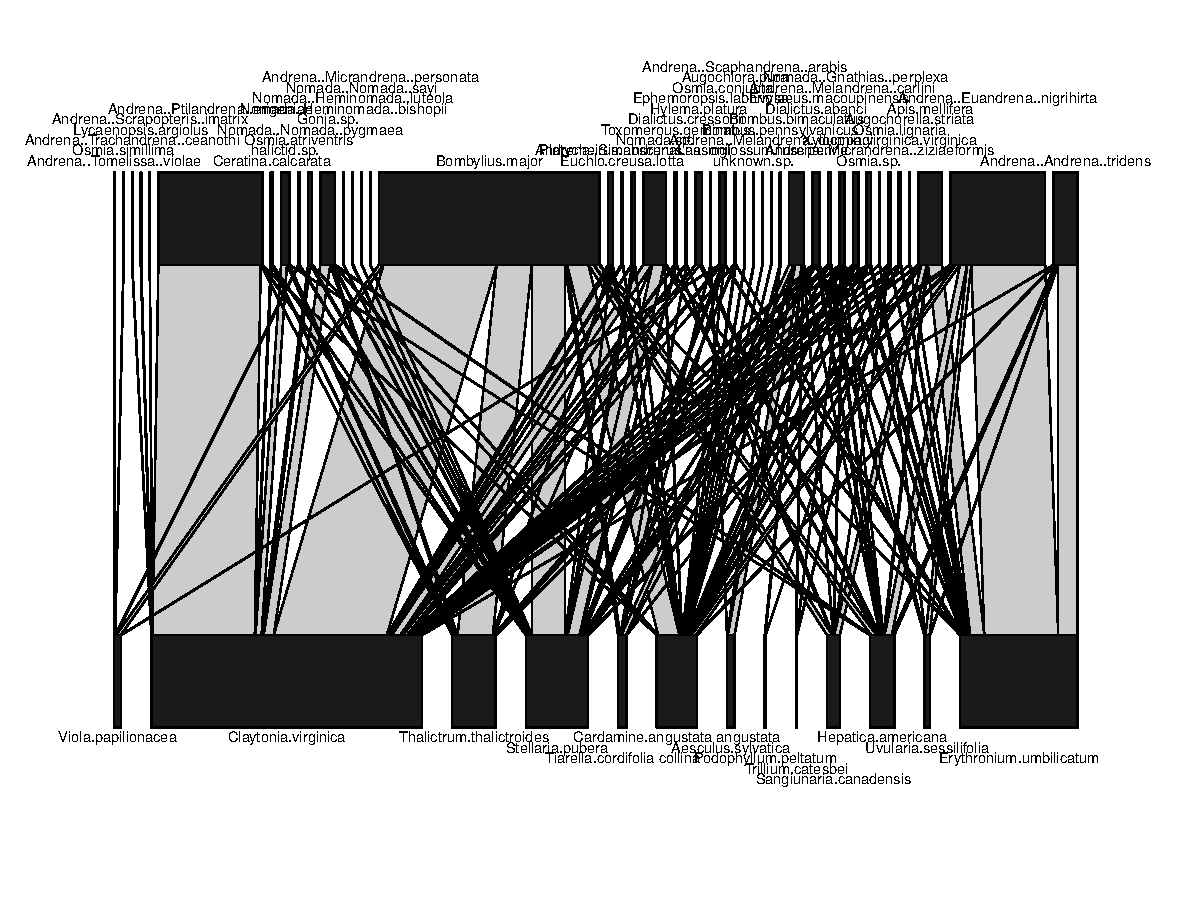
\includegraphics[width=0.7\textwidth]{figures/motten1982_plotweb}
	\smallskip
	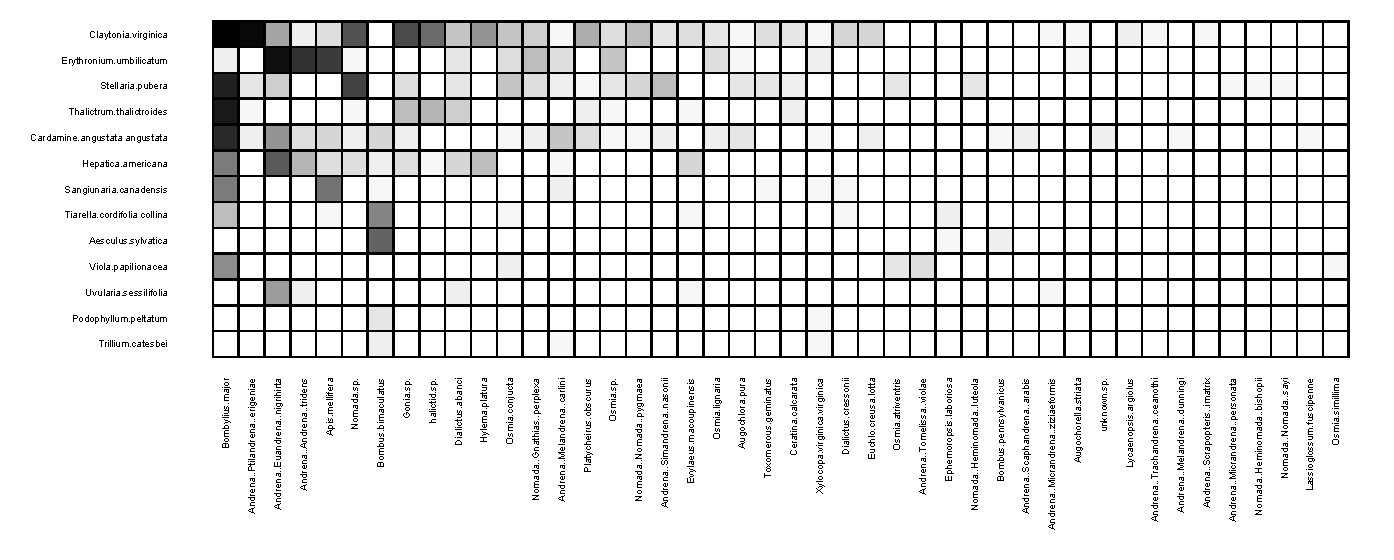
\includegraphics[width=0.7\textwidth]{figures/motten1982_visweb}
	\caption{A bipartite graph of Motten's (1982) pollination network (\emph{top}) and a visualisation of the adjacency matrix (\emph{bottom}). The darker a cell is represented, the more interactions have been observed. By default, \texttt{plotweb} minimises overlap of lines and \texttt{visweb} sorts by marginal totals.}
	\label{fig:Amotten}
\end{figure}



The function \indR{plotPAC} visualises  (Fig.~\ref{fig:AplotPAC}) a very special idea: the potential for apparent competition \citep{Morris2005}. The idea is that every parasitoid emerging from a host can attack another species. Thus, the more individuals emerge from a host, the larger is the potential for these to reduce the competition between hosts, as long as they choose their prey equiprobable. Pretty as it may be, its current value is highest for host-parasitoid networks, so the plot employing a pollination network is for illustration only.
\begin{Schunk}
\begin{Sinput}
> plotPAC(PAC(motten1982), outby=0.9)
\end{Sinput}
\end{Schunk}
%pdf(file="figures/motten1982_PACplot.pdf", width=3, height=3)
%plotPAC(PAC(motten1982), outby=0.9)
%dev.off()

\begin{wrapfigure}{o}{0.3\textwidth}
  \vspace{-2cm}
	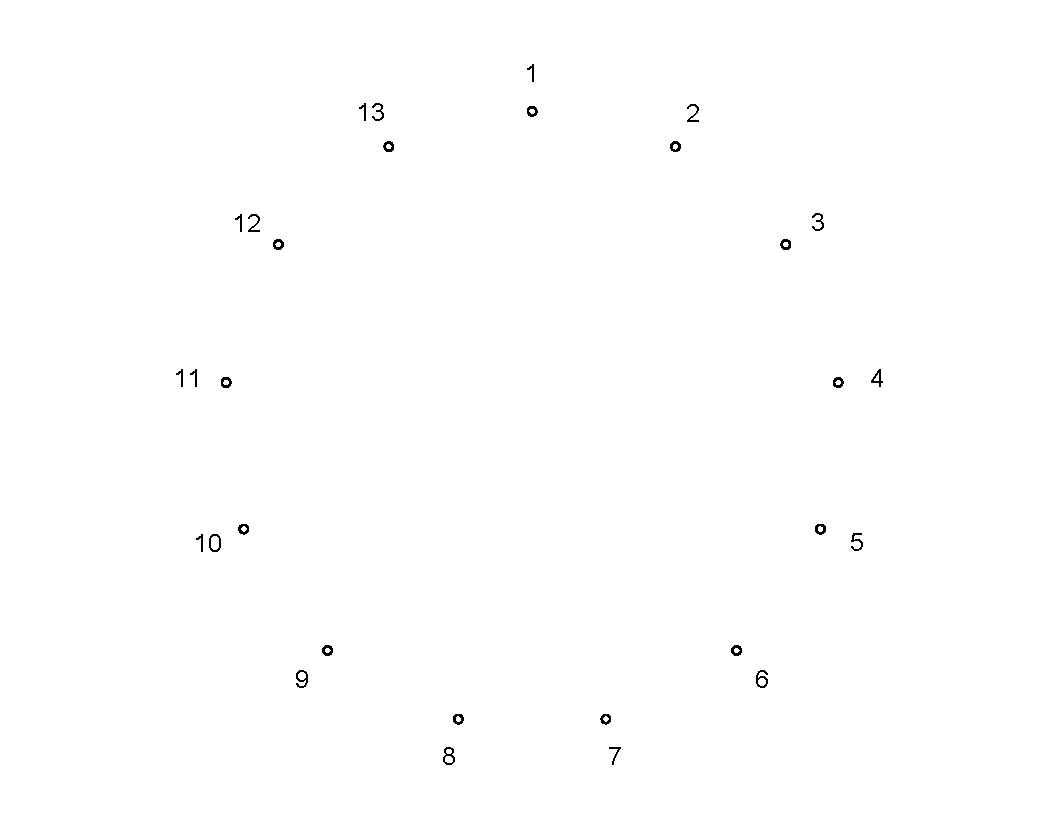
\includegraphics[width=0.3\textwidth]{figures/motten1982_PACplot}
	\caption{A PAC-plot of Motten's \citeyear{Motten1982} pollination network. Lines connect plants potentially visited next by a pollinator. Line width is proportional to probability, which is very similar in this example. See help of \emph{plotPAC} for details on plotting and meaning.}
	\label{fig:AplotPAC}
\end{wrapfigure}
%
We can also visualise communities within the network by computing its modularity and then plotting the result, using the functions \texttt{computeModules} and \texttt{plotModuleWeb}, respectively (Fig.~\ref{fig:Amoduleplot}).
\begin{Schunk}
\begin{Sinput}
> mod <- computeModules(motten1982)
> plotModuleWeb(mod)
\end{Sinput}
\end{Schunk}
%pdf(file="figures/motten1982_moduleplot.pdf", width=12, height=7)
%plotModuleWeb(mod)
%dev.off()
\begin{figure}%[h]
\centering
	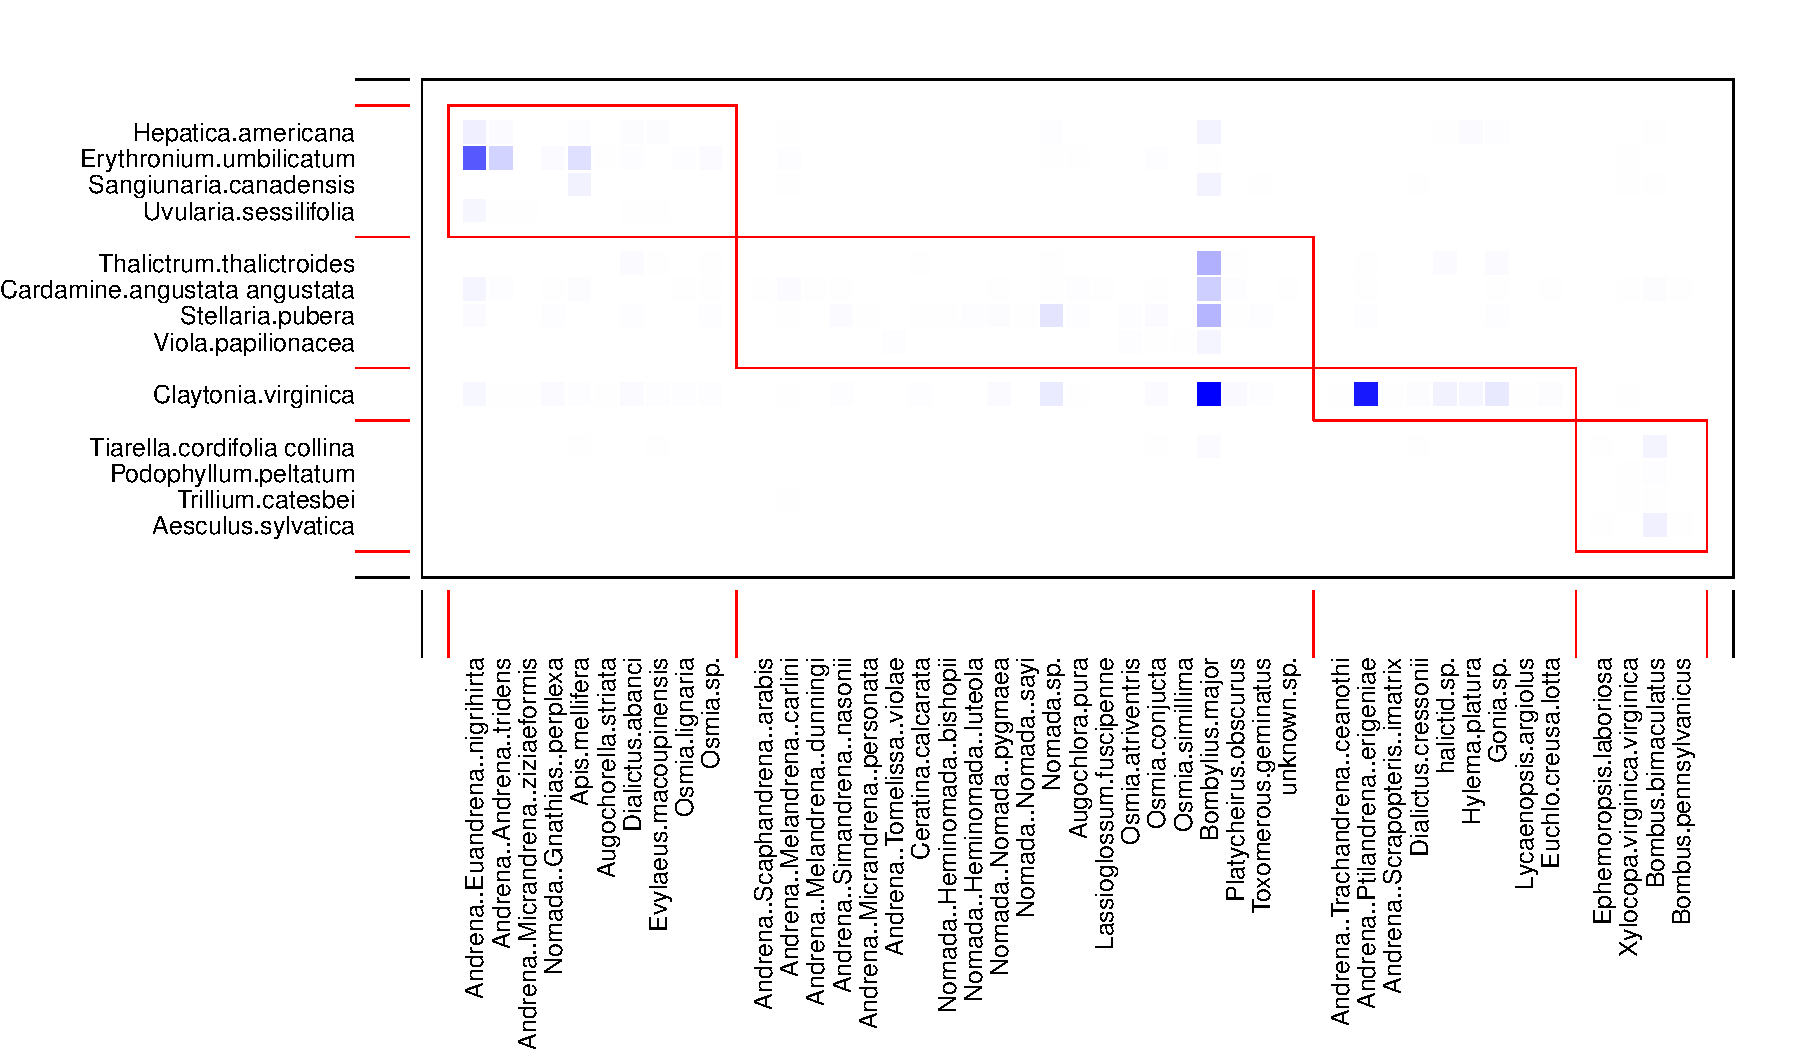
\includegraphics[width=0.7\textwidth]{figures/motten1982_moduleplot}
	\caption{The adjacency matrix of Motten's (1982) pollination network, organised into modules.}
	\label{fig:Amoduleplot}
\end{figure}
%
To visualise either level separately projected into one-mode mode, we have to employ a different package, for example \package{sna} \citep{Butts2013}. We can do the projection on the fly, though. For networks with even a moderate number o species, such plots can become rather obtuse and uninformative (Fig.~\ref{fig:Amottengplot} top).
\begin{Schunk}
\begin{Sinput}
> par(mfrow=c(1,2), xpd=T)
> gplot(as.one.mode(motten1982, project="higher"), 
+  label=colnames(motten1982), gmode="graph", 
+ label.cex=0.6, vertex.cex=2)
> gplot(as.one.mode(motten1982, project="lower"), 
+ 	label=rownames(motten1982), gmode="graph", 
+ 	label.cex=0.6, vertex.cex=2, vertex.col="green")
\end{Sinput}
\end{Schunk}
%pdf(file="figures/motten1982_gplot.pdf", width=14, height=7)
%par(mfrow=c(1,2), xpd=T)
%gplot(as.one.mode(motten1982, project="higher"), 
% label=colnames(motten1982), gmode="graph", 
%label.cex=0.6, vertex.cex=2)
%
%gplot(as.one.mode(motten1982, project="lower"), 
%	label=rownames(motten1982), gmode="graph", 
%	label.cex=0.6, vertex.cex=2, vertex.col="green")
%dev.off()
%
\begin{wrapfigure}{o}{1\textwidth}
\centering
	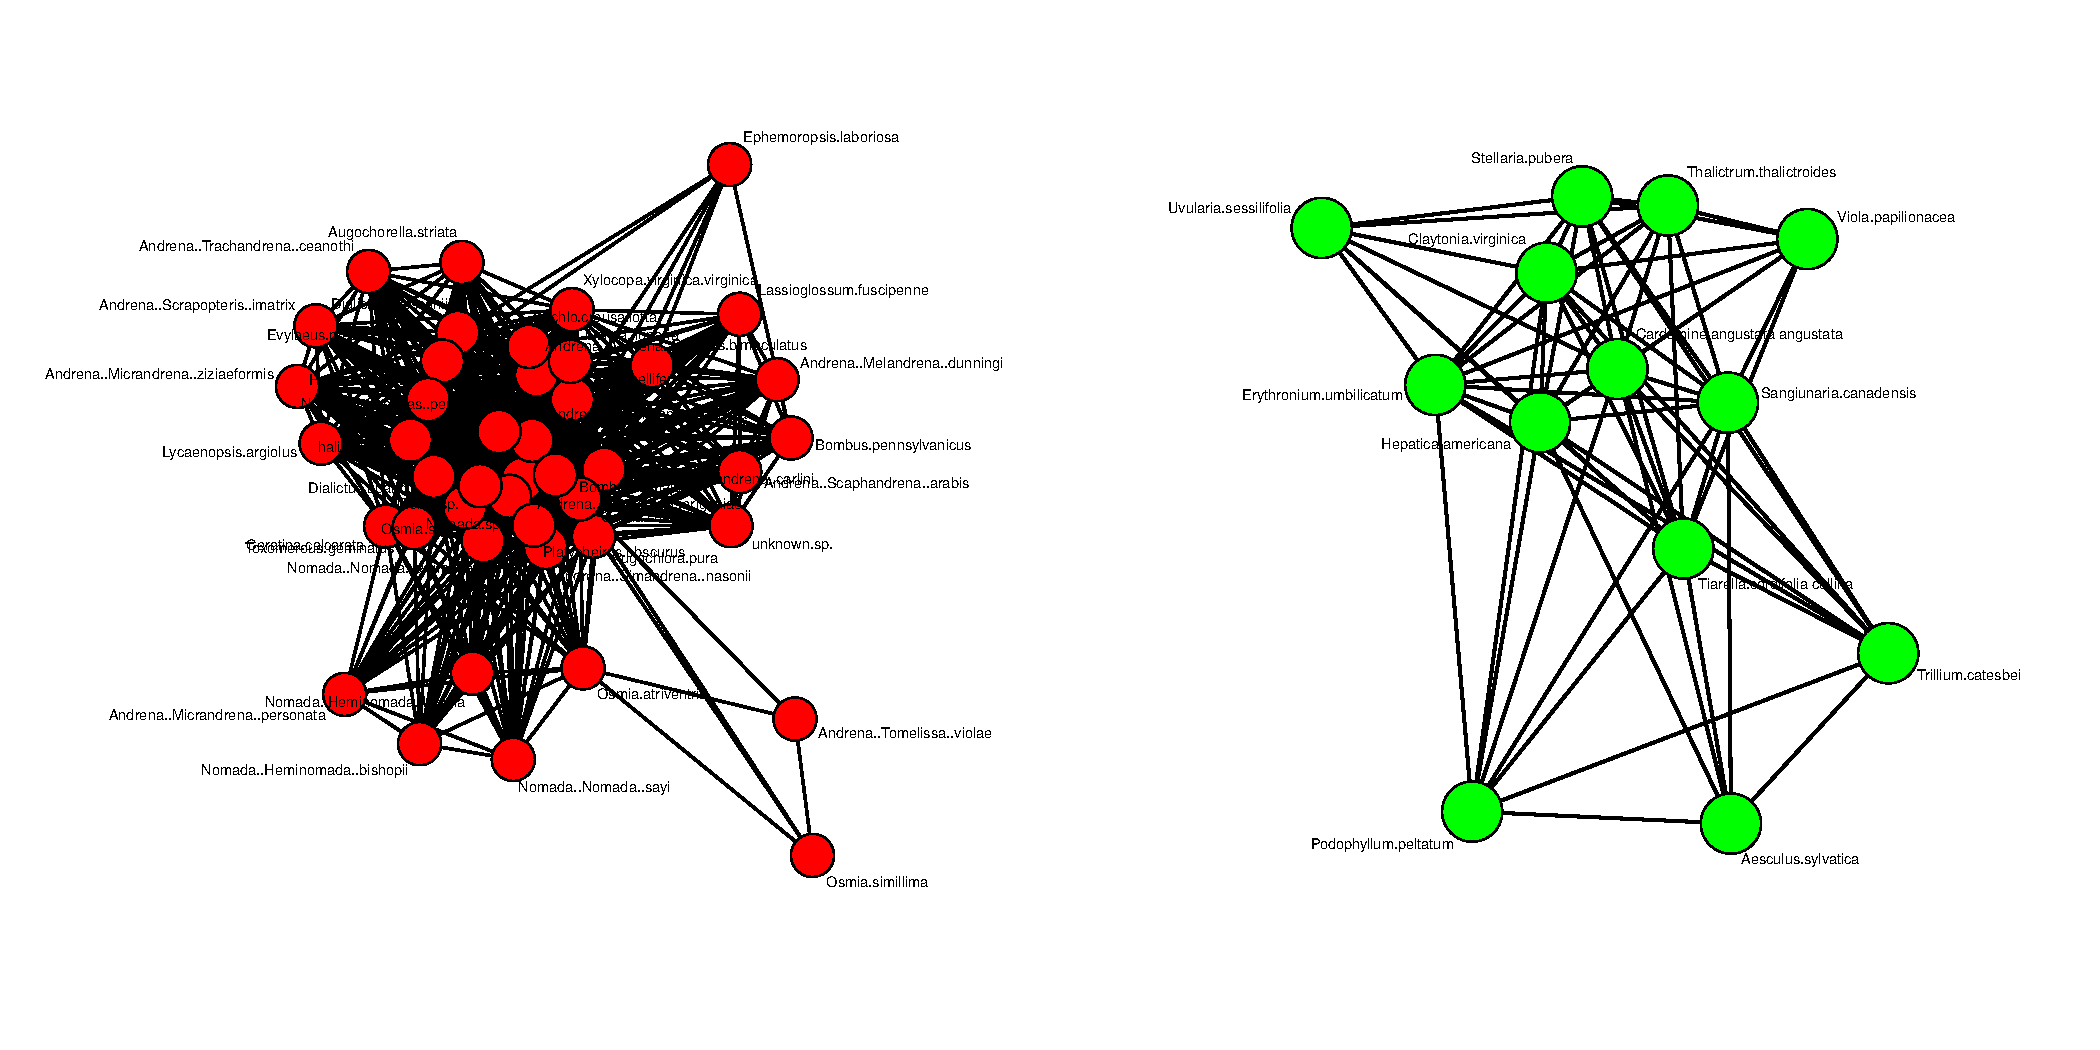
\includegraphics[width=0.9\textwidth]{figures/motten1982_gplot}
	\caption{Plots of one-mode projections of Motten's (1982) pollination network. Pollinators in red (\emph{top}), plants in green (\emph{bottom}). Note that these plots are point-symmetrically variable, hence every plot will look somewhat different.}
	\label{fig:Amottengplot}
\end{wrapfigure}


\clearpage

\section{Computing indices} %--------------------------------------------------------------------
Network indices are primarily that: metrics to quantify an aspect of the network. Each may have a justification, a purpose, but the information in a matrix is only finite. As a consequence, network indices are highly correlated. There is thus no point in computing all indices in the book; rather should we consider very carefully what we want to test with the data and select one (or a few) indices to do so.

The \package{bipartite}-package offers itself to data dredging: with one function one can compute dozens of indices, certainly some of them will be significantly correlated with whatever we want to test. While analyses are commonly carried out in this way, this is obviously statistically inappropriate. Two issues are important here. One is that of multiple testing, and there are dozens of publications covering this issue. The other is an attempt to formalise one's expectation. Null models are one way to do so, in particular one's expectation of what a pattern is like in the \emph{absence} of a process. This technical details of this topic are covered further below (section \ref{sec:A:nullmodels}). 

Indices (currently) come at the following hierarchical levels:
\begin{enumerate}
\item network-level (a single value, per index, for the entire network);
\item group-level  (a value, per index, for each of the two groups);
\item link-level  (a value, per index, for each edge = link);
\item node-level (a value, per index, for each node = species); and
\item species-level (a value, per index, for each species).
\end{enumerate}



\subsection{Network-level indices}\label{networklevel}
This set of indices is computed for the entire network. They are called using the function \indR{networklevel}, which additionally (and conveniently) makes available all indices from the group level, too. Those restricted to the network-level are:
\begin{enumerate}
\item \texttt{\ind{connectance}}, also called `standardised number of species combinations' in biogeographic analyses \citep{Gotelli1996, Dunne2002};
\item \texttt{web asymmetry}, the balance of the number of species in the two levels \citep{Bluethgen2007}; 
\item \texttt{links per species};
\item \texttt{number of compartments};
\item \texttt{compartment diversity} \citep{Tylianakis2007};
\item \texttt{cluster coefficient}, which will compute both the network-wide binary, one-mode-based cluster coefficient as well as those for each level,
\item \texttt{nestedness}, with the returned value indicating the `temperature' of the matrix, which is low ($0$) for a perfectly nested matrix \citep{RodriguezGirones2006};
\item \texttt{weighted nestedness}, or more specifically `weighted interaction nestedness estimator' (WINE), with $1$ indicating perfected nestedness (thus exactly opposite to the previous index) \citep{Galeano2009a};
\item \texttt{weighted NODF}, as an alternative measure of quantitative nestedness, automatically correcting for matrix filling and also indicating nestedness by values towards $1$ \citep{AlmeidaNeto2011}; 
\item \texttt{interaction strength asymmetry} \citep{Bluethgen2007} \citep[or alternatively \texttt{ISA} or \texttt{dependence asymmetry}][]{Bascompte2003}, which quantify whether specialised species interacts with generalised ones in the other level (or vice versa);
\item \texttt{specialisation asymmetry} (or alternatively \texttt{SA}), following the same idea as the previous, but this being based on species specialisation in $d'$;
\item \texttt{linkage density}, marginal totals-weighted diversity of interactions per species \citep{Bersier2002};
\item \texttt{Fisher alpha}, diversity index based on fitting a Fisher-series \citep{Fisher1943};
\item \texttt{interaction evenness}  quantifies how balanced the distribution of interactions is across species, based on Shannon's diversity \citep{Tylianakis2007};
\item \indR{Alatalo interaction evenness}, as an alternative measure of interaction evenness, attempting to overcome some of the shortcomings of the previous, Shannon's, version \citep{Alatalo1981,Muller1999};
\item \texttt{Shannon diversity};
\item \texttt{H2}, network-wide specialisation index $H_2'$ \citep{Bluethgen2006}.
\end{enumerate}

\noindent Similarly to the previous sets of indices, several options are available to fine-tune those in \texttt{networklevel}:
\begin{Schunk}
\begin{Sinput}
> networklevel(bezerra2009, index=c("ISA", "weighted NODF", "Fisher alpha"), SAmethod="log")
\end{Sinput}
\begin{Soutput}
                 weighted NODF interaction strength asymmetry 
                  5.717160e+01                   8.842823e-05 
                  Fisher alpha 
                  8.793400e+00 
\end{Soutput}
\end{Schunk}





\subsection{Group-level indices}\label{grouplevel}
Indices that can be computed for each group separately are collected in the function \indR{grouplevel}.\footnote{If network-level indices are also desired, all indices in \texttt{grouplevel} are also accessible through \texttt{networklevel}, see below.} Quite a few of these indices are aggregates from the species level (e.g. by averaging species' degrees), in which case the mean is weighted by the number of observations of each species, thus giving more weight to species for which information is more reliable.\footnote{The weighting can be switched off by stating \texttt{weighted=FALSE}.} Others are biogeographic indices which change their value when the matrix is inverted (i.e. when a group changes from ``species'' to ``islands''). The following indices are implemented:
\begin{enumerate}
\item \texttt{number of species} in the respective trophic level;
\item \texttt{mean number of links};
\item \texttt{mean number of shared partners} \citep{Roberts1990,Stone1992}; 
\item \texttt{cluster coefficient}, which supposedly informs us whether a network has `small world' properties \citep{Watts1998};
\item \texttt{weighted cluster coefficient}, which takes into account the number of interactions and is a properly derived bipartite version of the previous one-mode cluster coefficent above \citep{Opsahl2010};
\item \texttt{togetherness} as the mean number of co-occurrences across all pairwise species combinations \citep{Stone1992};
\item \texttt{\ind{C score}}, or `checkerboardness', which averages the number of instances of 01/10-patterns (i.e. exclusive occurrences) for all pairwise species combinations \citep{Stone1990};
\item \texttt{\ind{V ratio}}, the variance ratio of species numbers to interaction numbers within species of a level \citep{Schluter1984};
\item \texttt{\ind{discrepancy}}, the number of links one would have to move to achieve perfect nestedness \citep{Brualdi1999};
\item \texttt{degree distribution}, fitting an exponential function and (truncated) power laws\citep{Jordano2003};
\item \texttt{extinction slope}, with different options for the extinction sequence \citep{Memmott2004};
\item \texttt{robustness}, the area under the extinction curve \citep{Burgos2007};
\item \texttt{niche overlap}, with options for distance metrics \citep{Pielou1972,Hurlbert1978};
\item \texttt{\ind{generality}} (for the higher trophic level) or \texttt{\ind{vulnerability}} (for the lower one) \citep{Bersier2002};
\item \texttt{partner diversity}, simply the mean Shannon diversity of interactions of each species in a level;
\item \texttt{effective partners} as before, but as the exponent of the base to which Shannon was computed (typically $e$ or $2$) \citep{Jost2006};
\item \texttt{fd} (or alternatively \texttt{\ind{functional diversity}}), which is similar to niche overlap but computed as branch length of a cluster diagram of dissimilarity of resource use \citep{Devoto2012}.
\end{enumerate}

\noindent As in the case of species-level indices, some allow for normalisation (between 0 and 1), others for different basis to the logarithm or similar tuning. A typical call to \texttt{grouplevel} will thus comprise the list of desired indices\footnote{Or alternatively the argument \texttt{index="ALL"}.} and their options, as well as the level(s) for which the computation shall be carried out:
\begin{Schunk}
\begin{Sinput}
> grouplevel(bezerra2009, level="both", index=c("mean number of links", "weighted 
+      cluster coefficient", "effective partners", "niche overlap"), dist="bray")
\end{Sinput}
\begin{Soutput}
mean.number.of.links.HL mean.number.of.links.LL        niche.overlap.HL 
              9.9502551               7.0975057               0.2824538 
       niche.overlap.LL           generality.HL        vulnerability.LL 
              0.4795595               8.0590841               5.6963672 
\end{Soutput}
\end{Schunk}
The LL and HL behind each index indicate that it was computed for the lower and higher level, respectively. A relatively comprehensive comparison of network-level indices \citep{Dormann2009}, including some at the group level, has shown substantial redundancy among these indices, and few of them have a sound theoretical basis.



\subsection{Node-level indices}\label{nodelevel}
...



\subsection{Link-level indices}\label{linklevel}
At the moment, only few indices have been investigated at the level of the individual link (i.e. the cell of a network matrix):
\begin{enumerate}
\item dependence \citep[i.e. the relevance of each species for the other level][]{Bascompte2006} one matrix for each level;
\item endpoint degree \citep[i.e. product of degrees of species linked by this cell][]{Barrat2004}.
\end{enumerate}
It is employed by simply applying it to the network under consideration and selecting the index desired:
\begin{Schunk}
\begin{Sinput}
> str(linklevel(bezerra2009, index=c("dependence", "endpoint")))
\end{Sinput}
\begin{Soutput}
List of 3
 $ HL dependence: num [1:13, 1:13] 0.193 0.131 0.056 0.108 0.105 ...
  ..- attr(*, "dimnames")=List of 2
  .. ..$ : chr [1:13] "Diplopterys.pubipetala" "Byrsonima.gardnerana" "Banisteriopsis.muricata" "Heteropterys.sp1" ...
  .. ..$ : chr [1:13] "Centris.aenea" "Centris.fuscata" "Centris.caxiensis" "Centris.tarsata" ...
 $ LL dependence: num [1:13, 1:13] 0.2415 0.2238 0.0997 0.2474 0.2632 ...
  ..- attr(*, "dimnames")=List of 2
  .. ..$ : chr [1:13] "Diplopterys.pubipetala" "Byrsonima.gardnerana" "Banisteriopsis.muricata" "Heteropterys.sp1" ...
  .. ..$ : chr [1:13] "Centris.aenea" "Centris.fuscata" "Centris.caxiensis" "Centris.tarsata" ...
 $ endpoint     : num [1:13, 1:13] 117 78 156 104 91 65 52 26 52 52 ...
  ..- attr(*, "dimnames")=List of 2
  .. ..$ : chr [1:13] "Diplopterys.pubipetala" "Byrsonima.gardnerana" "Banisteriopsis.muricata" "Heteropterys.sp1" ...
  .. ..$ : chr [1:13] "Centris.aenea" "Centris.fuscata" "Centris.caxiensis" "Centris.tarsata" ...
\end{Soutput}
\end{Schunk}
This function is so rudimentary, and its output so disproportionally voluminous, that it is not worth going into further details here and use \texttt{str} to only show the structure of the output.




\subsection{Species-level indices}\label{specieslevel}
The (growing) list of indices computable for each species in the network comprises (the index name to be used in the call is given in \texttt{typewriter} font):
\begin{enumerate}
\item \texttt{degree}, i.e. the number of links of each species,
\item \texttt{normalised degree} for a normalised version of degree \citep{MartinGonzalez2010},
\item \texttt{species strength} as sum of dependencies for each species \citep{Bascompte2006},
\item \indR{nestedrank} as rank in a nested matrix \citep{Alarcon2008},
\item \texttt{interaction} for interaction push/pull (a version of dependence asymmetry), \citep{Vazquez2007},
\item \texttt{PDI} for \ind{Paired Differences Index} \citep{Poisot2011,Poisot2011a},
\item \indR{resource range} for Schoener's index of unused resources \citep{Schoener1989},
\item \texttt{species specificity} (or coefficient of variation of interactions) \citep{Julliard2006,Poisot2012a},
\item \texttt{PSI} for \ind{pollination service index} (or pollinator support index, depending on the trophic level),\footnote{devised by the author with Nico Blüthgen and Bernd Gruber}
\item \texttt{NS} for \ind{node specialisation index} \citep{Dalsgaard2008},
\item \indR{betweenness} for betweenness \citep{Borgatti1997},
\item \indR{closeness} (both automatically also return their weighted counterparts proposed by Tore Opsahl in package \package{tnet}),
\item \texttt{Fisher} for \ind{Fisher's alpha} as a measure of diversity \citep{Fisher1943},
\item \texttt{diversity} for Shannon diversity of interactions of that species,
\item \texttt{effective partners} for the effective number of interacting partners \citep{Bersier2002},
\item \texttt{proportional generality} for a quantitative version of normalised degree,\footnote{devised by Jochen Fründ}
\item \texttt{proportional similarity} as specialisation measured as similarity between use and availability \citep{Feinsinger1981},
\item \texttt{d} for Blüthgen's $d'$ \citep{Bluethgen2006}.
\end{enumerate}

\noindent Some of them allow for normalisation (between 0 and 1), others for different basis to the logarithm or similar tuning. A typical call to \texttt{specieslevel} will thus comprise the list of desired indices\footnote{Or alternatively the argument \texttt{index="ALL"}.} and their options, as well as the level(s) for which the computation shall be carried out:
\begin{Schunk}
\begin{Sinput}
> specieslevel(bezerra2009, level="lower", index=c("normalised degree", "PDI", 
+       "effective partners"), PDI.normalise=F)
\end{Sinput}
\begin{Soutput}
                           normalised.degree       PDI effective.partners
Diplopterys.pubipetala             0.6923077 1010.0000           7.437631
Byrsonima.gardnerana               0.4615385 1939.6667           3.819660
Banisteriopsis.muricata            0.9230769  657.0000           9.191488
Heteropterys.sp1                   0.6153846  570.3333           6.278285
Heteropterys.sp2                   0.5384615  567.3333           5.865968
Dicella.bracteosa                  0.3846154  429.0000           4.582040
Carolus.chasei                     0.3076923  513.6667           3.751208
Stigmaphyllon.paralias             0.1538462  774.0000           1.944388
Banisteriopsis.stellaris           0.3076923  245.6667           3.787887
Banisteriopsis.schizoptera         0.3076923  189.0000           3.822392
Stigmaphyllon.auriculatum          0.3076923  204.3333           3.687447
Stigmaphyllon.ciliatum             0.2307692  238.0000           2.937197
Janusia.anisandra                  0.2307692  220.3333           2.813322
\end{Soutput}
\end{Schunk}
A relatively comprehensive comparison of species-level indices of specialisation \citep{Dormann2011} has shown substantial redundancy among these indices, and few of them have a sound theoretical basis \cite{Poisot2012a}.



\subsection{Which index to chooose?}%--------------------------------------------------------------
Different indices were invented (``developed'') for different purposes. However, for most indices, it has not been demonstrated that they actually achieve what their inventor had in mind. Most commonly indices quantify a specific pattern which may have come about by a whole variety of different causes. Take, for example, connectance, i.e. the proportion of possible links actually recorded. Low connectance may be caused by high specialisation or by low samplng intensity. The same holds true for a species' degree, which (typically) increases with sampling effort as well as generalisation. For the choice of an index this means that we cannot solely rely on what the inventor has proposed this index to be good for, but we have to keep in mind that it may actually quantify several other things, too.

Apart from the different levels at which an index can quantify a network pattern (from the individual link to the entire network, as covered in sections \ref{linklevel}--\ref{networklevel}), indices can be divided into those for binary and those for weighted data (called here binary and weighted indices, respectively). Binary indices only use the information of whether a link exists, while weighted indices additionally account for how strong a link is, as judged from the actual value in a network matrix.%\footnote{This is the difference between graph $\vec{A}$ and graph $\vec{B}$ in section \ref{sec:graphtheory}.}

Binary indices, by definition, use less information. It does not follow that they are thus more robust! In fact, \citet{Bluethgen2010} argues the opposite, since only a weighted index can tell whether an observed value indicates specialisation or not.\footnote{Imagine two species, one with entries (1, 1), the other with entries (1, 100). A binary index would not be able to tell between them, while a quantitative would expose the second as far more specialised.} 

This, if two indices are available to quantify the same idea, one binary and one quantitative, one should generally choose the quantitative one. Rather than species degree, we should use species strength or linkage density. Table \ref{tab:binaryquantitative} depicts some such binary-quantitative index pairs.
%
\begin{table}
\label{tab:binaryquantitative}
\caption{Binary-quantitative pairs of network indices. Note: Most quantitative indices can also be computed on binary networks. That does not make them a quantitative measure!}
\begin{tabular}{l|ll}
\hline
& binary & quantitative \\ \hline
%link level    & --     & --           \\ \hline
network level & connectance & $H_2'$\\ 
& links per species & linkage density \\ 
& nestedness        & weighted NODF, wine \\ %\hline
group level   & mean number of partners & effective number of partners \\%\hline
species level & degree & species strength, effective number of partners \\\hline
\end{tabular}
\end{table}


In a nutshell: Quantitative indices make use of more information in the data. They are generally more advisable, although most of them also are strongly affected by sampling issues.



\subsubsection{Index redundancy: do different indices tell the same thing?}
%Redundancy and similarity of indices -> PCA/nMDS; clustering

To visualise the similarity and possible redundancy of the different indices, they are computed for the networks in \package{bipartite} and summarised through a principal component analysis (see Fig.~\ref{fig:PCAnetworklevel}).
\begin{Schunk}
\begin{Sinput}
> web.names <- data(package="bipartite")$results[,3]
> data(list=web.names) #loads all webs
> # the next step takes around 10 minutes:
> netw.indic.webs <- t(sapply(web.names, function(x) networklevel(get(x), index="ALLBUTDD")))
\end{Sinput}
\end{Schunk}
% save(PCA.out, netw.indic.webs, file="figures/netw.indic.webs.Rdata")
\begin{Schunk}
\begin{Sinput}
> PCA.out <- prcomp(netw.indic.webs[,-5], scale.=T)
> biplot(PCA.out, xpd=T, las=1)
> summary(PCA.out)
\end{Sinput}
\begin{Soutput}
Importance of components:
                          PC1    PC2     PC3     PC4     PC5     PC6    PC7
Standard deviation     4.2780 3.6461 2.09732 1.84163 1.32612 1.09350 1.0375
Proportion of Variance 0.3979 0.2890 0.09562 0.07373 0.03823 0.02599 0.0234
Cumulative Proportion  0.3979 0.6869 0.78248 0.85621 0.89444 0.92044 0.9438
                           PC8     PC9    PC10    PC11    PC12    PC13    PC14
Standard deviation     0.81058 0.64158 0.62560 0.56960 0.49217 0.43179 0.36230
Proportion of Variance 0.01428 0.00895 0.00851 0.00705 0.00527 0.00405 0.00285
Cumulative Proportion  0.95812 0.96707 0.97558 0.98263 0.98789 0.99195 0.99480
                          PC15    PC16   PC17    PC18    PC19    PC20      PC21
Standard deviation     0.26591 0.25249 0.2254 0.18080 0.11401 0.09049 7.038e-16
Proportion of Variance 0.00154 0.00139 0.0011 0.00071 0.00028 0.00018 0.000e+00
Cumulative Proportion  0.99634 0.99772 0.9988 0.99954 0.99982 1.00000 1.000e+00
\end{Soutput}
\end{Schunk}
%pdf(file="figures/PCAnetworklevel.pdf", width=7, height=7)
%biplot(PCA.out, xpd=T, las=1)
%dev.off()

Apparently 40, 30 and 10\% of the variation in indices can be partitioned to the first three axes. We can now investigate which indices load on the first two axes:
\begin{Schunk}
\begin{Sinput}
> round(PCA.out$rotation[, 1:6], 3)
\end{Sinput}
\begin{Soutput}
                                        PC1    PC2    PC3    PC4    PC5    PC6
connectance                           0.177  0.147 -0.044  0.025  0.231 -0.046
web asymmetry                        -0.137 -0.098 -0.298  0.063 -0.123 -0.046
links per species                     0.189 -0.087 -0.020  0.183 -0.171 -0.131
number of compartments               -0.147  0.005  0.167 -0.051 -0.008 -0.252
cluster coefficient                   0.169  0.128  0.005  0.119  0.261 -0.114
nestedness                           -0.020  0.196 -0.004  0.305  0.264  0.034
weighted nestedness                   0.066 -0.108 -0.170 -0.399 -0.148  0.139
weighted NODF                         0.193  0.068 -0.138 -0.182  0.024  0.038
interaction strength asymmetry       -0.172  0.080 -0.178 -0.028  0.049 -0.252
specialisation asymmetry              0.021  0.109  0.337 -0.096 -0.138  0.077
linkage density                       0.049 -0.258 -0.058 -0.038  0.108  0.058
Fisher alpha                         -0.041 -0.246  0.045 -0.053  0.234 -0.028
Shannon diversity                     0.073 -0.251  0.011  0.082  0.048  0.021
interaction evenness                  0.179 -0.078  0.012  0.102  0.246  0.111
Alatalo interaction evenness          0.076  0.159  0.143 -0.045  0.443  0.078
H2                                   -0.191  0.089  0.091  0.037 -0.054 -0.226
number.of.species.HL                 -0.048 -0.249  0.026 -0.062  0.199 -0.027
number.of.species.LL                 -0.020 -0.256  0.121 -0.038  0.057 -0.048
mean.number.of.partners.shared.in.HL  0.191 -0.032 -0.177  0.189 -0.113 -0.077
mean.number.of.partners.shared.in.LL  0.218  0.042 -0.049 -0.042  0.076 -0.227
cluster.coefficient.HL                0.189  0.093 -0.001 -0.036  0.011  0.259
cluster.coefficient.LL                0.155  0.085 -0.285 -0.009  0.072  0.075
weighted.cluster.coefficient.HL       0.150 -0.122 -0.189  0.162 -0.181 -0.086
weighted.cluster.coefficient.LL       0.212 -0.040  0.035  0.145 -0.134 -0.064
niche.overlap.HL                      0.045  0.142 -0.287 -0.272  0.014  0.028
niche.overlap.LL                      0.202  0.035  0.062 -0.195 -0.007  0.159
togetherness.HL                       0.023  0.181 -0.283 -0.032  0.159  0.061
togetherness.LL                       0.216  0.052  0.087 -0.041  0.137 -0.066
C.score.HL                           -0.162 -0.123  0.217  0.147 -0.042  0.045
C.score.LL                           -0.216 -0.020  0.038  0.026  0.087 -0.142
V.ratio.HL                            0.177 -0.121  0.121 -0.101 -0.222 -0.087
V.ratio.LL                           -0.048 -0.238 -0.151 -0.113  0.005  0.024
discrepancy.HL                       -0.041 -0.251  0.059 -0.042  0.183 -0.036
discrepancy.LL                       -0.039 -0.252  0.062 -0.037  0.175 -0.032
extinction.slope.HL                   0.216 -0.006  0.063  0.131  0.025 -0.093
extinction.slope.LL                   0.120 -0.061  0.035  0.326  0.079 -0.167
robustness.HL                         0.214 -0.020  0.059  0.148 -0.046  0.029
robustness.LL                         0.150 -0.084 -0.114  0.254 -0.220 -0.068
functional.diversity.HL               0.162  0.003  0.027 -0.257  0.031 -0.471
functional.diversity.LL               0.163 -0.003  0.029 -0.259  0.036 -0.465
partner.diversity.HL                  0.198 -0.078  0.183 -0.028 -0.063  0.158
partner.diversity.LL                  0.061 -0.222 -0.212  0.082  0.064  0.043
effective.partners.HL                 0.187 -0.079  0.206 -0.101 -0.049  0.090
effective.partners.LL                -0.003 -0.256 -0.125 -0.011  0.132  0.036
generality.HL                         0.187 -0.079  0.206 -0.101 -0.049  0.090
vulnerability.LL                     -0.003 -0.256 -0.125 -0.011  0.132  0.036
\end{Soutput}
\end{Schunk}
As we can see, there are quite a few indices on the first axis with a loading of around 0.2 (links per species, weighted NODF, H2, mean number of partners shared; weighted cluster coefficient, niche overlap, togetherness, C-score (all lower level); extinction slope, robustness, partner diversity (all higher level)). 

Also the PCA biplot is not very helpful, since the many indices pointing ``southwards'' are unreadably overlapping.
%
\begin{figure}
%\vspace*{1cm} 
\centering
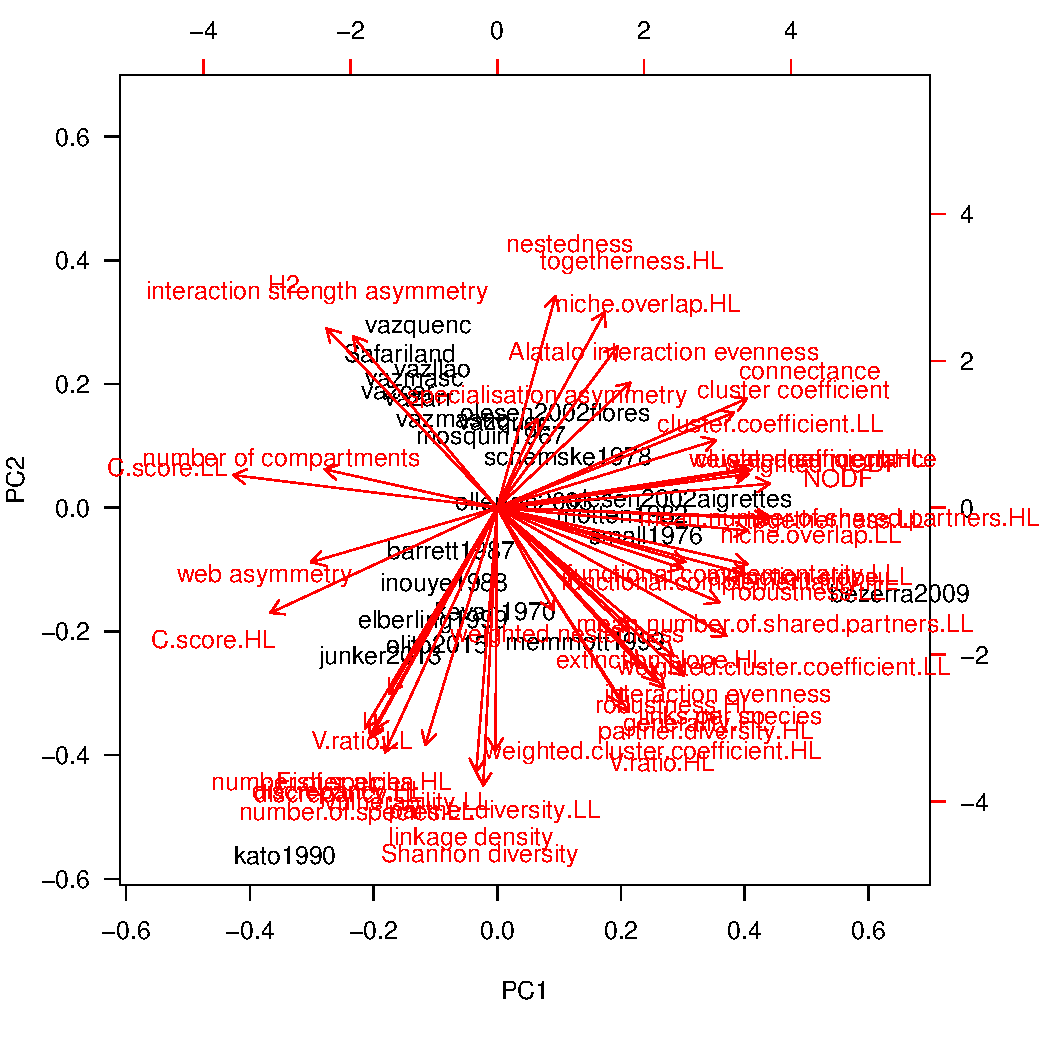
\includegraphics[width=0.8\textwidth]{figures/PCAnetworklevel}
\caption{Principal component analysis biplot of indices at the network level, based on 22 quantitative pollination networks. Notice that network ``kato1990'' is by far the largest in the set, defining on its own the second principal component. Indices pointing ``southwards'' may thus simply be more sensitive to network size and related properties (such as density of interactions).}
\label{fig:PCAnetworklevel}
\end{figure}


Alternatively, we might want to depict the correlation between different indices by means of a cluster analysis (Fig.~\ref{fig:clusternetworklevel}).
%par(mar=c(0,5,0,0))
\begin{Schunk}
\begin{Sinput}
> library(Hmisc)
> plot(varclus(netw.indic.webs), cex=0.8)
> abline(h=0.5, lty=2, col="grey")
\end{Sinput}
\end{Schunk}
%pdf(file="figures/clusternetworklevel.pdf", width=10, height=7)
%par(mar=c(4,5,1,1))
%plot(varclus(netw.indic.webs), cex=0.8)
%abline(h=0.5, lty=2, col="grey")
%dev.off()
\begin{figure}
\centering
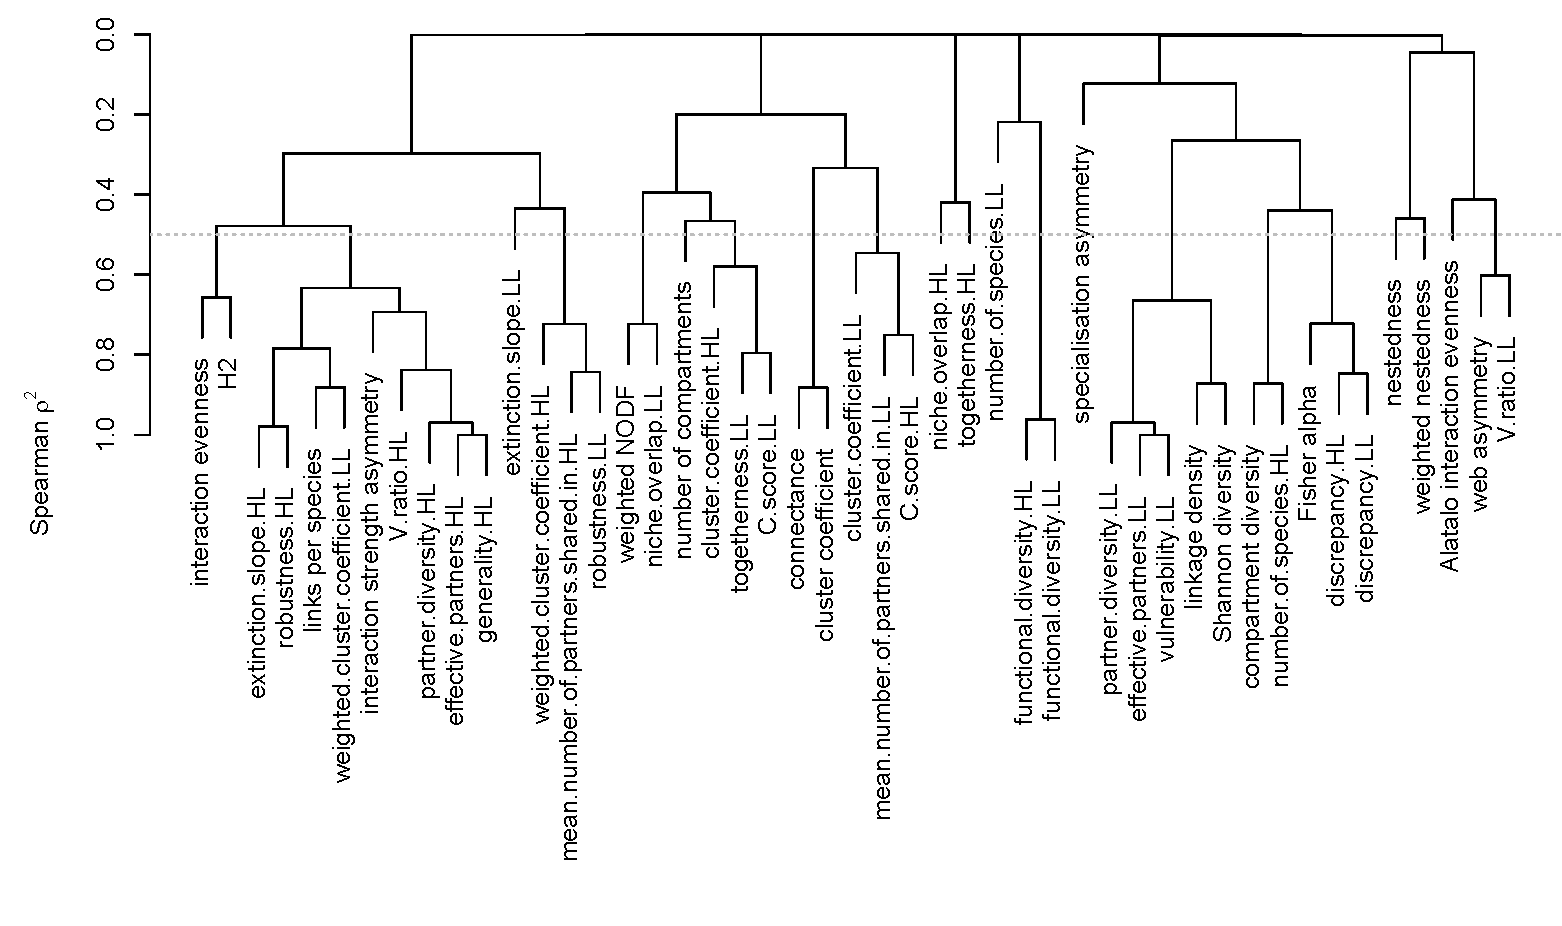
\includegraphics[width=0.8\textwidth]{figures/clusternetworklevel}
\caption{Cluster analysis of indices at the network level, based on 22 quantitative pollination networks. Grey dotted line indicates the level below which clustering could be considered relevant ($|r| > 0.7$).}
\label{fig:clusternetworklevel}
\end{figure}
%
It picks out a slightly different structure, with the PC1 being distributed over more than one cluster (towards the left, with extinction.slope.HL but also towards the centre, with weighted NODF). In either case it becomes clear that many indices are of limited originality. However, there are some branches ending above the dashed line, indicating that they add a new element to the description of the network. Some are trivial, such as the number of species in the lower level, others less so (specialisation asymmetry, extinction slope LL, niche overlap HL, (weighted) nestedness). 

It should become clear that there is no need to compute all indices a software can offer, and that some clusters seem to measure the same latent property, even it is unclear what that property is. Curiously, higher and lower level indices are always intermixed. There seems to be always an effect onto the other level, so that some indices pick up a signal in one level, but others the same signal in the other.\footnote{That should be the case for extinction slopes and robustness, which measures the response of one level to extinctions in the other. But is difficult to see why the cluster coefficient for the higher level should be correlated with togetherness in the lower. \emph{Post hoc}, it is always possible to find a reason, but \emph{a priori} this is not expected.}

The 22 pollination networks, on which both PCA and cluster are based, are most certainly not representative of bipartite networks in general. The simulations of \citet{Dormann2009} for a wider range of sizes and linkage densities show a qualitatively similar picture, though: indices are overlapping into clusters.\footnote{We could similarly say that there is a substantial redundancy in network indices, evident from the analysis where we condense 92\% of variation in 40 odd indices onto six axes.}



\subsubsection{Variations on on the same theme: which index of a group of similar ones should I choose?}
%nestedness; graph-theoretical indices (closeness, betweenness, node specialisation);

%Close with: indices differently affected by uninformative (first-order) properties of the network: network dimensions, connectance, sampling intensity, ... -> null models needed for identifying the signal-to-noise ratio of different indices. -> next section

Different indices were developed for different aims. Some are very reasonable, logically sound, thoughtful and even productive (in the sense of ``shown to be doing what they are supposed to do''), others aren't. Each index should be understood when being used, based on the literature introducing it and any later study refining, comparing or criticising/appraising it. There is no easy way to decide the question ``Which is the right index for me?''

That said, there are a few guiding considerations that seem plausible to me:
\begin{enumerate}
\item Quantitative indices use more information than binary ones; preferably use the former.
\item Indices developed for bipartite networks are likely to be closer, theoretically, to the structure of the data than one-mode indices working on projections of bipartite networks.
\item Indices that came out positively in comparisons have proven their worth more than fresh-off-the-press indices.
\item If two or more indices seem barely distinguishable, do \textbf{not} choose the one easiest to interpret! This would be a logical fault, since their similarity indicates clearly that they are affected by ``something'' and we don't know what that something is, yet. But interpreting an effect as the being caused by what is most convenient to interpret is most certainly wrong \citep{Shermer2012}.\footnote{Of the many, many biases that can creep into scientific explorations, this is one. We could call it the ``parsimony bias'' as a special case of the ``selection bias'' \citep{Shermer2012}.}
\end{enumerate}
%
The last point in particular seems rather little helpful. Imagine the two index values ``functional diversity'' for the higher and lower trophic level, which are near-identical in Fig.~\ref{fig:clusternetworklevel}. This indicates that the \emph{network}, rather than each level, contains the information which these two indices describe. In this particular case, we may want to consider using neither index, or using any of them but interpreting it \emph{as if it represented \emph{both} level}.

Thus, in a nutshell, there is no easy answer and there is no way around knowing the index and the literature around it and its friends.





\section{Null models} %-------------------------------------------------------------------------
  \label{sec:nullmodels}

\subsection{Why null models?}
When a network is structured according to some measure (e.g. nestedness), what does that mean? It could mean that ecological processes leading to nestedness are at play. Or it could mean that a sampling effect makes nestedness an inevitable consequence. Or, finally, it could be a mixture of both. Furthering our understanding of nature is not aided by the reporting of spurious relationships resulting from sampling effects, hence a formal description of what the network would look like without the ecological process would be a useful comparison. That is what a null model aims to provide \citep{Gotelli1996}. 

In ecology, \ind{null model}s are common only in some fields, particularly in biogeography \citep{Gotelli1996,Hausdorf2007}, but also in network analyse \citep{Dormann2009,Joppa2009,Bluthgen2008,Vazquez2006,Vazquez2003a,Vazquez2009}. With respect to particular bipartite indices, some studies rejected the current nestedness paradigm using abundance-based null models, for observed \citep{Kallimanis2009,Moore2007,Santamaria2007}, as well as for simulated networks \citep{Krishna2008}.

Null models extend much beyond ecology and were probably first used in physics. \citet{Latapy2008} use them to investigate degree distributions in non-ecological bipartite networks. Using another network example, the module detection algorithm proposed by \citet{Newman2004} also uses a null model to define a ``group'' (or module or community) within a network: there are more links within than between groups. The null model then is a random network with as many links between as within groups \citep{Guimera2005}. In its quantitative version, the null model is constructed from equiprobable interactions by differently abundant participants \citep{Barber2004}. The specific null model used above is underlying most current implementations of contingency table tests such as $\chi^2$ or Fisher's signed rank test \citep{Patefield1981}.

In conclusion, null models are established approaches in physics as well as ecology to correct for statistical artefacts and to establish an expectation in the absence of the hypothesised structuring mechanism.

\subsection{Justifying conservative null models}
The interactions observed in a network are the result of a dynamic interaction between species at two levels. If we use null models to represent the outcome of these interactions (the abundances of the participants), we seem to be over-correcting. How can we possibly find a pattern, if we use this pattern as a null model? Is an abundance-based null model not a circular argument? Here I argue when it is not, and if \ind{circularity} would sneak in, why it would still be better to over-correct. I shall focus on pollination networks, and every network analyst has to decide in how far this reasoning can be applied to his/her system.

Plant persistence in a site depends to some extend on them being pollinated, and pollinator population dynamics is affected by the amount of nectar and pollen they collect from the flowers they visit. However, plant growth and population dynamics are also affected by nutrient and light availability, save sites for seed germination, herbivory and fungal pathogens, mycorrhisation and environmental disturbances; and similar constraints exist for pollinators. It is thus difficult, if not impossible, to say how much of the observed abundance of a species (plant or pollinator) is caused by the specific plant-pollinator interaction and hence the structure of the network. To the extent that abundances are determined by the pollination interaction we may indeed introduce collinearity. To date, there are no data to estimate the proportion of population growth controlled by mutualistic interactions of either plants or pollinators. We can only guess based on observations such as strong nest-site limitation in solitary bees \citep{SteffanDewenter2008}, relatively high parasitism rates of pollinators \citep{Klein2002}, strong nutrient limitations of plant population dynamics \citep{Ghazoul2005} and grazing pressure \citep{Crawley1987, deMazancourt2000} that they are probably not dominating population dynamics. On the other hand, clear (but rare) examples of co-evolution indicate that such a strong mutual dependence may indeed occur \citep{Waser1996,Waser2006}.

Secondly, the observed interactions are not necessarily reflecting abundance of flowers or pollinators, but rather their attractiveness (e.g. due to scent, colouration or nectar production) and activity (e.g. daily period of foraging, phenology through the season, temperature- dependence of foraging activity), respectively. Hence by using observed sums of observed interactions, one does not correct for abundance, but for attractiveness and activity, respectively.

Third, the null model uses marginal totals, i.e. summed across all links of a species. If a pollinator was specialised on a single plant species, the null model would scatter these interactions across all and hence correctly identify a miss-match between observed and null model. If, on the other hand, a pollinator was generalised, then the scattering of interactions across all plant species would also yield a similar picture and generalisation would correctly be inferred.

Finally, even if the null model used would introduce some amount of circularity and thus ``over-correction'', we have to balance this against ``over-detection''. Finding specialisation in an uncorrected approach will incur high levels of type I error (i.e. detecting a pattern that is actually not there). A null model insures against this type of error. We can thus be sure that a pattern that ``survives'' the null model test is no statistical artefact. Since it has been shown repeatedly that sampling intensity and ``natural'' differences in abundance will cause such artefacts \citep{Dormann2009,Bluthgen2010,Joppa2009,Bluthgen2008}, they must be addressed. Ignoring them will lead to misinterpretation and over-reporting of spurious network structure. After correction for expectation based on abundances, we can start understanding ecology \citep{Vazquez2007}.

In conclusion, circularity is unlikely to substantially impair null models for pollination networks. The risk of reporting non-existent network structure and further speculation of network stability due to this spurious network structure is a problem that requires a correction, even if circularity was present.



\subsection{Using null models to test for significant tests in data}\label{sec:A:nullmodels}
Once you have settled on a null model, there are fundamentally two different approaches to use such null models in statistical significance testing: corrected indices and null modelling the entire analysis. Let us look at them in turn, starting with the seemingly easier option.

\paragraph{Corrected indices and $z$-scores}\index{z-score@$z$-score}
Imagine we computed the index $I$ for a network. We now want to know whether this value is anything special, given the abundances of the species.\footnote{Thereby we justify the use of the Patefield algorithm as null model. But the approach is independent of which null model we use.} So we build, say, 1000 null models\footnote{E.g. using \texttt{nulls <- nullmodel(web=Safariland, N=1000, method='r2d')}} 
and compute our index $I$ for each of them. We can visualise the distribution of null-model $I$-values relative to our observed index value \citep{Dormann2009}.
\begin{Schunk}
\begin{Sinput}
> data(Safariland)
> Iobs <- C.score(Safariland)
> nulls <- nullmodel(web=Safariland, N=1000, method='r2d')
> Inulls <- sapply(nulls, C.score)
> plot(density(Inulls), xlim=c(0, 1), lwd=2)
> abline(v=Iobs, col="red", lwd=2)
\end{Sinput}
\end{Schunk}

\begin{figure}
\centering
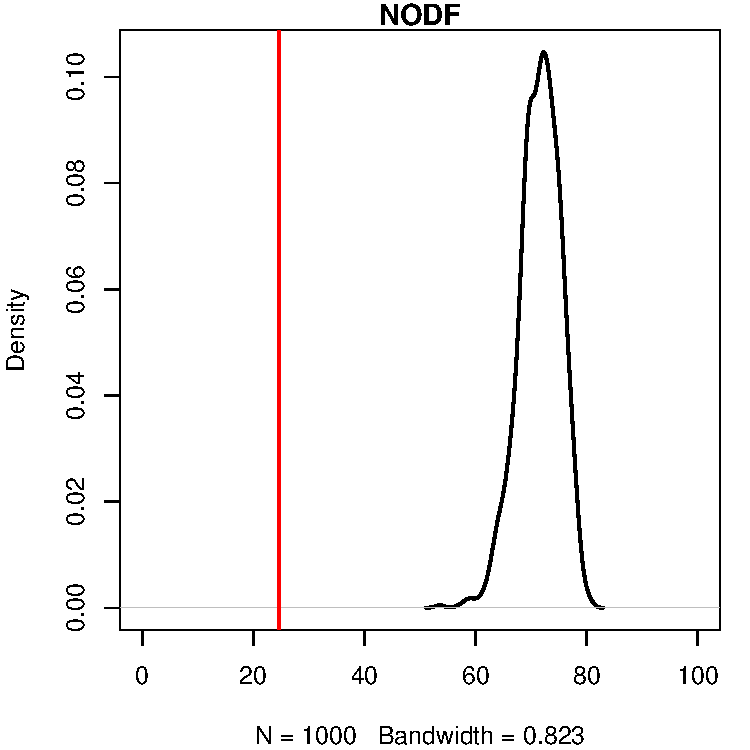
\includegraphics[width=0.5\textwidth]{figures/NODFnull}
\caption{Observed and null-modelled NODF-nestedness for the network vazquenc. Note that values of 100 indicate perfect nestedness. Thus, null models are much more nested than the observed network. (That is typically the case (Dormann et al. 2009), although typically no null models are computed for comparison.)}
\label{fig:NODFnull}
\end{figure}
%
That is fine for a single network, but no option if we want to analyse dozens or hundreds of networks. We thus have to summarise this figure in a value. The simplest, most obvious but generally not best solution would be to subtract the null model mean from the observed, so that $I_\text{corrected} = \Delta I= I_\text{observed} - \bar{I}_\text{nulls}$. The reason why this $\Delta I$ is not ideal is that the null model distribution is likely to vary from network to network. Thus, a difference of, say, 20 may be a lot for pointy distributed null models such as the one in Fig.~\ref{fig:NODFnull}, but only little for null model values spreading over the entire $x$-axis.

The better, and more established approach, would be to compute $z$-scores (= \ind{standard score}s or \ind{normal score}s) for each network, which express the difference in terms of standard deviations of the null distribution: 
\[z_I= \frac{I_\text{observed} - \bar{I}_\text{nulls}}{\sigma_{I_\text{nulls}}}.\] We can now analyse the $z$-scores instead of the original $I_\text{obs}$-values.

$z$-scores have one major disadvantage when it comes to several of the network indices presented earlier: the standard deviation becomes an unsuitable measure of spread as the values approach an upper or lower bound. Imagine our network index $I$ is bound between 0 and 1 (as many are). If the null models have values above, say, 0.9, the upper bound is so close that the distribution will be skewed and the standard deviation biased too low. This may lead to inflated $z$-scores. So whenever you observe values close to either bound, beware of distorted $z$-scores.
% show this in an example!


\paragraph{Null-model the entire analysis}
%(with a distribution of model estimates to compute p-values)
The alternative approach is to carry out the intended analysis on the observed index values $I$ and then, in a second step, repeat it with one realisation of a null model per network. Next, repeat this second step several thousand times (for good measure) and store the statistics you are interested in (say $F$-values in an ANOVA or slopes in a regression). Instead of using the $p$-values from the analysis of the observed values, compare observed and null-modelled statistics and count the proportion of values exceeding the observed and use those as $p$-value. To anyone with any experience in \ind{resampling analysis} or bootstrapping this is standard procedure \citep{Efron1993,Manly1997}.
% provide an example: e.g. Diego's analysis of with/out cattle on some index

As an example, we can use a question addressed in \citet{Vazquez2003}, where the authors investigate whether cattle grazing affects the network structure of pollination networks in four replicated sites in Argentina. As response we can choose any network index, for example linkage density. %or weighted NODF? or ISA? or effective number of species

\begin{Schunk}
\begin{Sinput}
> weblist <- lapply(c("Safariland", "vazarr", "vazllao", "vazcer", "vazmasc", 
+                        "vazmasnc", "vazquec", "vazquenc"), get)
> # Write a function to compute the desired statistic, e.g. the difference 
> # between grazed and ungrazed:
> meandiff <- function(webs){
+    obs <- sapply(webs, networklevel, index="linkage density")  
+    mean(obs[1:4] - obs[5:8])
+ }
> (observed <- meandiff(weblist))
\end{Sinput}
\begin{Soutput}
[1] -0.2481145
\end{Soutput}
\end{Schunk}
Now generate a null model and repeat:\index{nullmodel@\texttt{nullmodel}}
\begin{Schunk}
\begin{Sinput}
> nulllist <- lapply(weblist, nullmodel, N=1, method="r2d")
> meandiff(weblist)
\end{Sinput}
\begin{Soutput}
[1] -0.2481145
\end{Soutput}
\end{Schunk}
Repeat this procedure, say, 5000 times:\footnote{For didactic purposes, we use an inelegant but easy to understand \texttt{for}-loop here. In productive mode we would instead use \texttt{sapply} or \texttt{replicate}, which would make the code more compact, but in this case not faster.}\index{for-loop@\texttt{for}-loop}
\begin{Schunk}
\begin{Sinput}
> res <- 1:5000
> for (i in 1:5000){ # takes a few minutes !!
+    nulllist <- sapply(weblist, nullmodel, N=1, method="r2d")
+    res[i] <- meandiff(nulllist)  
+ }
\end{Sinput}
\end{Schunk}
Finally, we can depict the results in a histogram (Fig.~\ref{fig:cattlenull}), with observed as vertical line, and compute the $p$-value based on the 5000 null models:
%
\begin{figure}
\centering
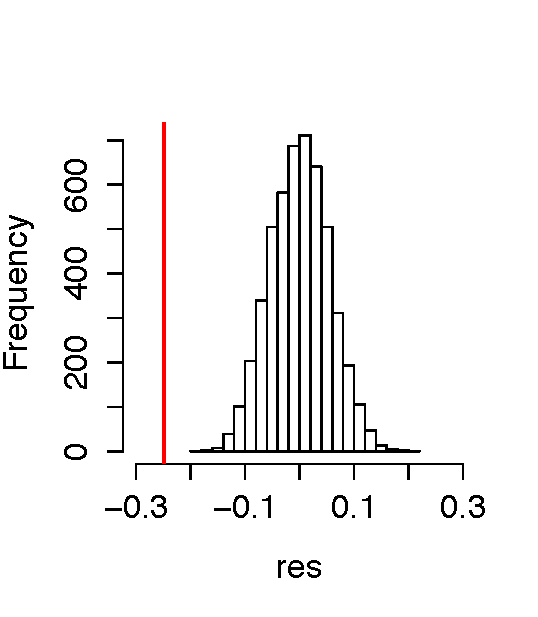
\includegraphics[width=0.5\textwidth]{figures/cattle_nullmodelled}
\caption{Distribution of mean differences in linkage density of pollination networks in grazed and ungrazed meadows, correcting for differences in species numbers and observation intensity through the use of null models ($N=5000$). Observed difference is shown as vertical line. The observed difference is significantly ($P<0.001$) different from null model expectations.}
\label{fig:cattlenull}
\end{figure}
%
\begin{Schunk}
\begin{Sinput}
> hist(res, xlim=c(-0.3, 0.3))
> abline(v=observed, col="red", lwd=2)
> # compute p-value as proportion smaller or than observed
\end{Sinput}
\end{Schunk}
\begin{Schunk}
\begin{Sinput}
> sum(res < observed)/length(res) * 2 # *2 for two-tailed test
\end{Sinput}
\begin{Soutput}
[1] 0
\end{Soutput}
\end{Schunk}
The idea here is to compute a statistic of interest, in this case the mean difference between some network index for the two treatments, and then use the null model to compute expectations. In the above example, we would apparently expect no difference (which is intuitive); additionally we also get an idea of how much variability we can expect (the distribution of the null model-based mean differences in linkage density). Thus, in this example, the difference in linkage density of pollination networks from grazed \emph{vs} ungrazed pastures is highly significant ($p<0.001$).


\section{Modularity}
Aggregated sets of interacting species are called `modules'. Their defining feature is that \emph{within}-module interactions are more prevalent than \emph{between}-module interactions \citep{Newman2003,Newman2004,Fortunato2010}. In other words, modules are link-rich clusters of species in a community. The package \package{bipartite} offers an algorithm \citep[QuaBiMo, described in technical detail here in][]{Dormann2013} to detect modules in bipartite networks, taking into account the quantitative nature of links. The algorithm has been vastly improved by \citep{Beckett2016}, which is also now the default algorithm used in \package{bipartite}.

An alternative to finding and delimiting such modules is to group species by ordination \citep{Borgatti1997,Lewinsohn2006}. Correspondence analysis (CA) of the adjacency matrix is a simple and fast way to organise species. In fact, the \package{bipartite}'s functions \texttt{plotweb} and \texttt{visweb} both use CA to decide on the species sequence, thereby grouping species of one group interacting similarly with species in the other group near each other. 
Typically, however, correspondence analysis will not be able to identify modules sufficiently well, even if modules are actually compartments (i.e. perfectly separated: Fig.~\ref{fig:randomCAsorted} left, centre). The algorithm used in \package{bipartite} can do so, at least in principle (Fig.~\ref{fig:randomCAsorted} right).\footnote{As a note on terminology: If modules are perfectly separated, with no species interacting with species in another module, they are called compartments and will be visible as clearly separated groups of species. It is relatively straightforward to implement a recursive compartment detection function, but compartments are much more black-and-white than modules and often only occur in ecological networks because sampling was rather incomplete.}
\begin{figure}
	\hfill
	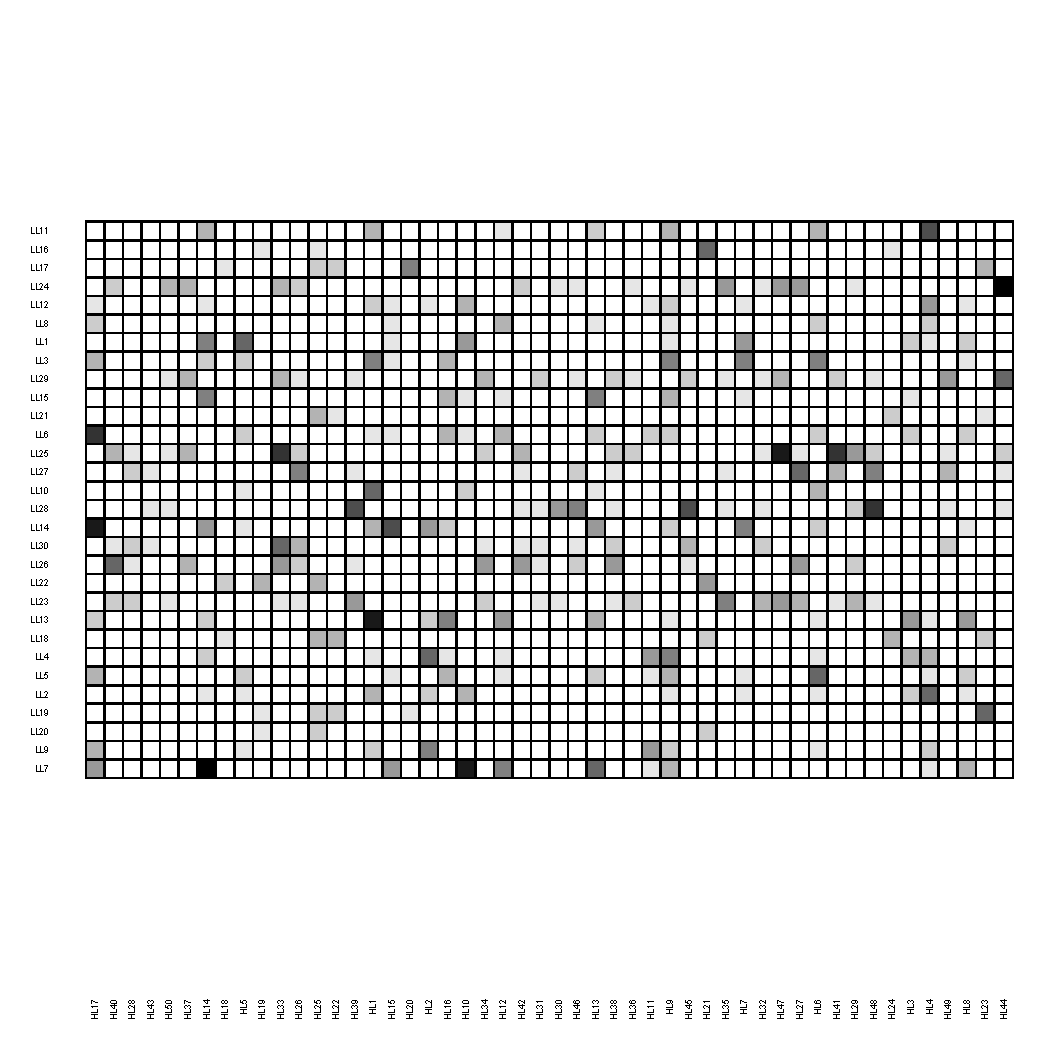
\includegraphics[width=0.32\textwidth, trim=1cm 4cm 0.5cm 1cm, clip=TRUE]{figures/random_small_high_nonoise}
	\hfill
	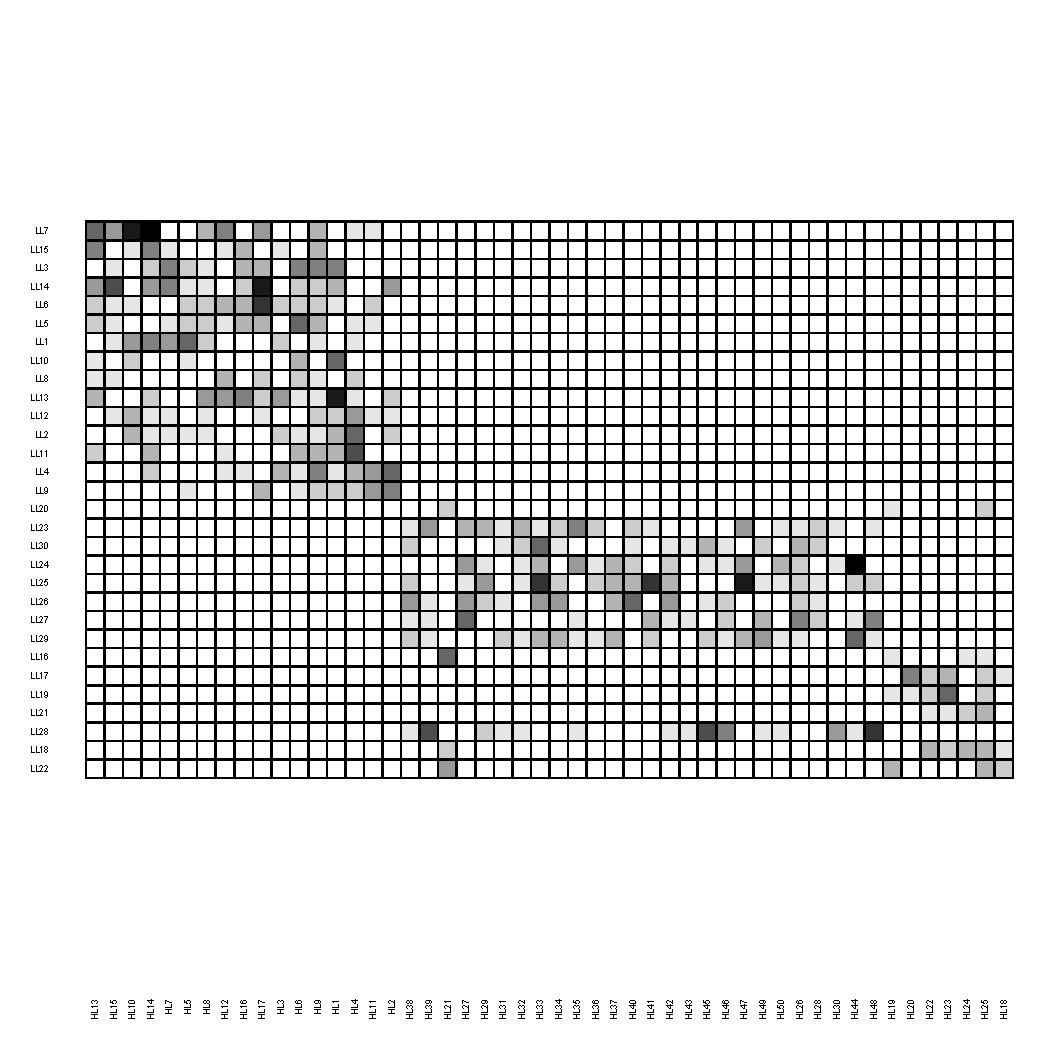
\includegraphics[width=0.32\textwidth, trim=1cm 4cm 0.5cm 1cm, clip=TRUE]{figures/CA_small_high_nonoise}
	\hfill
	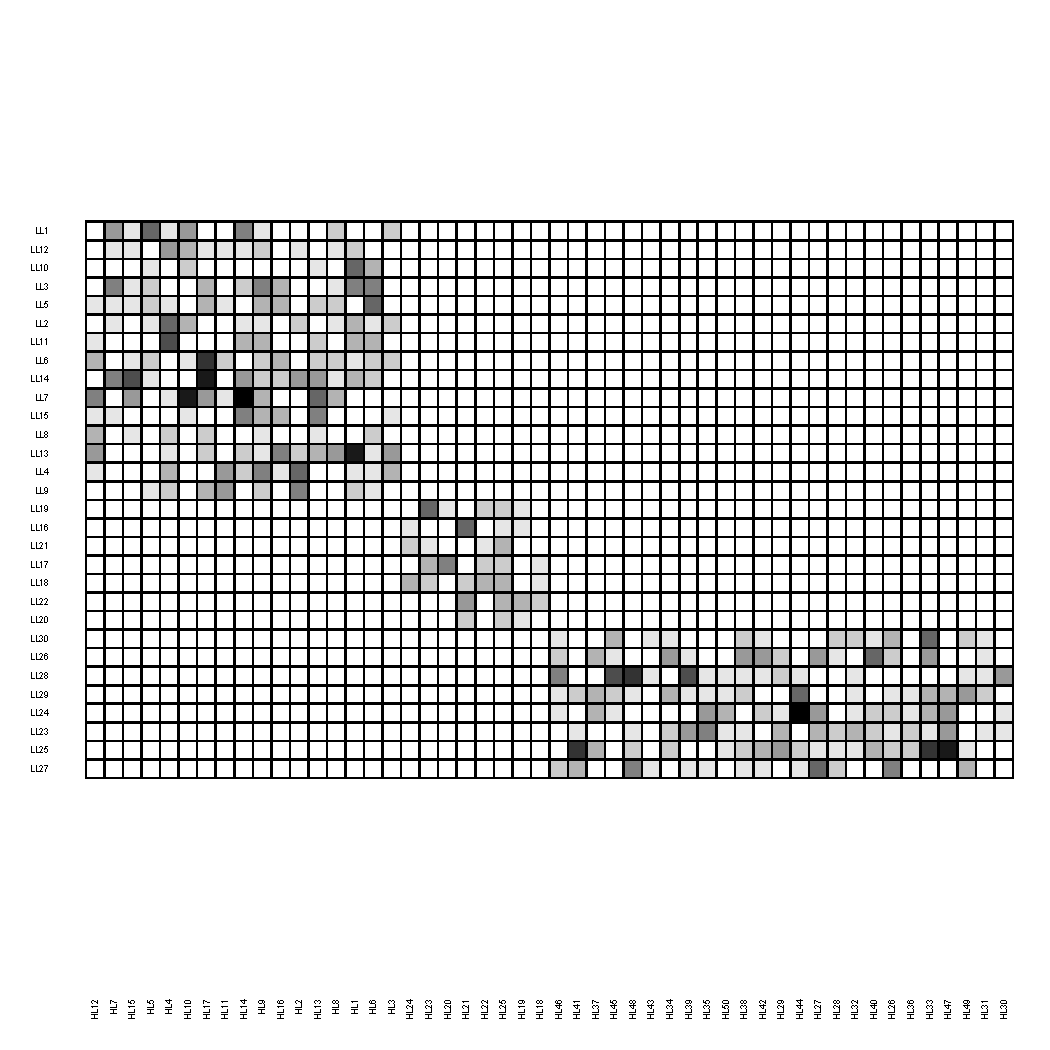
\includegraphics[width=0.32\textwidth, trim=1cm 4cm 0.5cm 1cm, clip=TRUE]{figures/sorted_small_high_nonoise}
	\hfill
	\caption{A simulated 3-compartment network in random sequence (left), as sorted by a correspondence analysis (centre) and by the modularity algorithm with default settings (right).}
\label{fig:randomCAsorted}
\end{figure}

QuaBiMo can be invoked recursively (we are working on doing the same for Beckett), searching for modules within modules (Fig.~\ref{fig:memmottmodules}, bottom). While such nested modules become ever smaller and are thus ever faster to detect, there are plenty of them and hence nesting will typically dramatically prolong computing time during the search for patterns \citep{Memmott1999}.
\begin{figure}
	%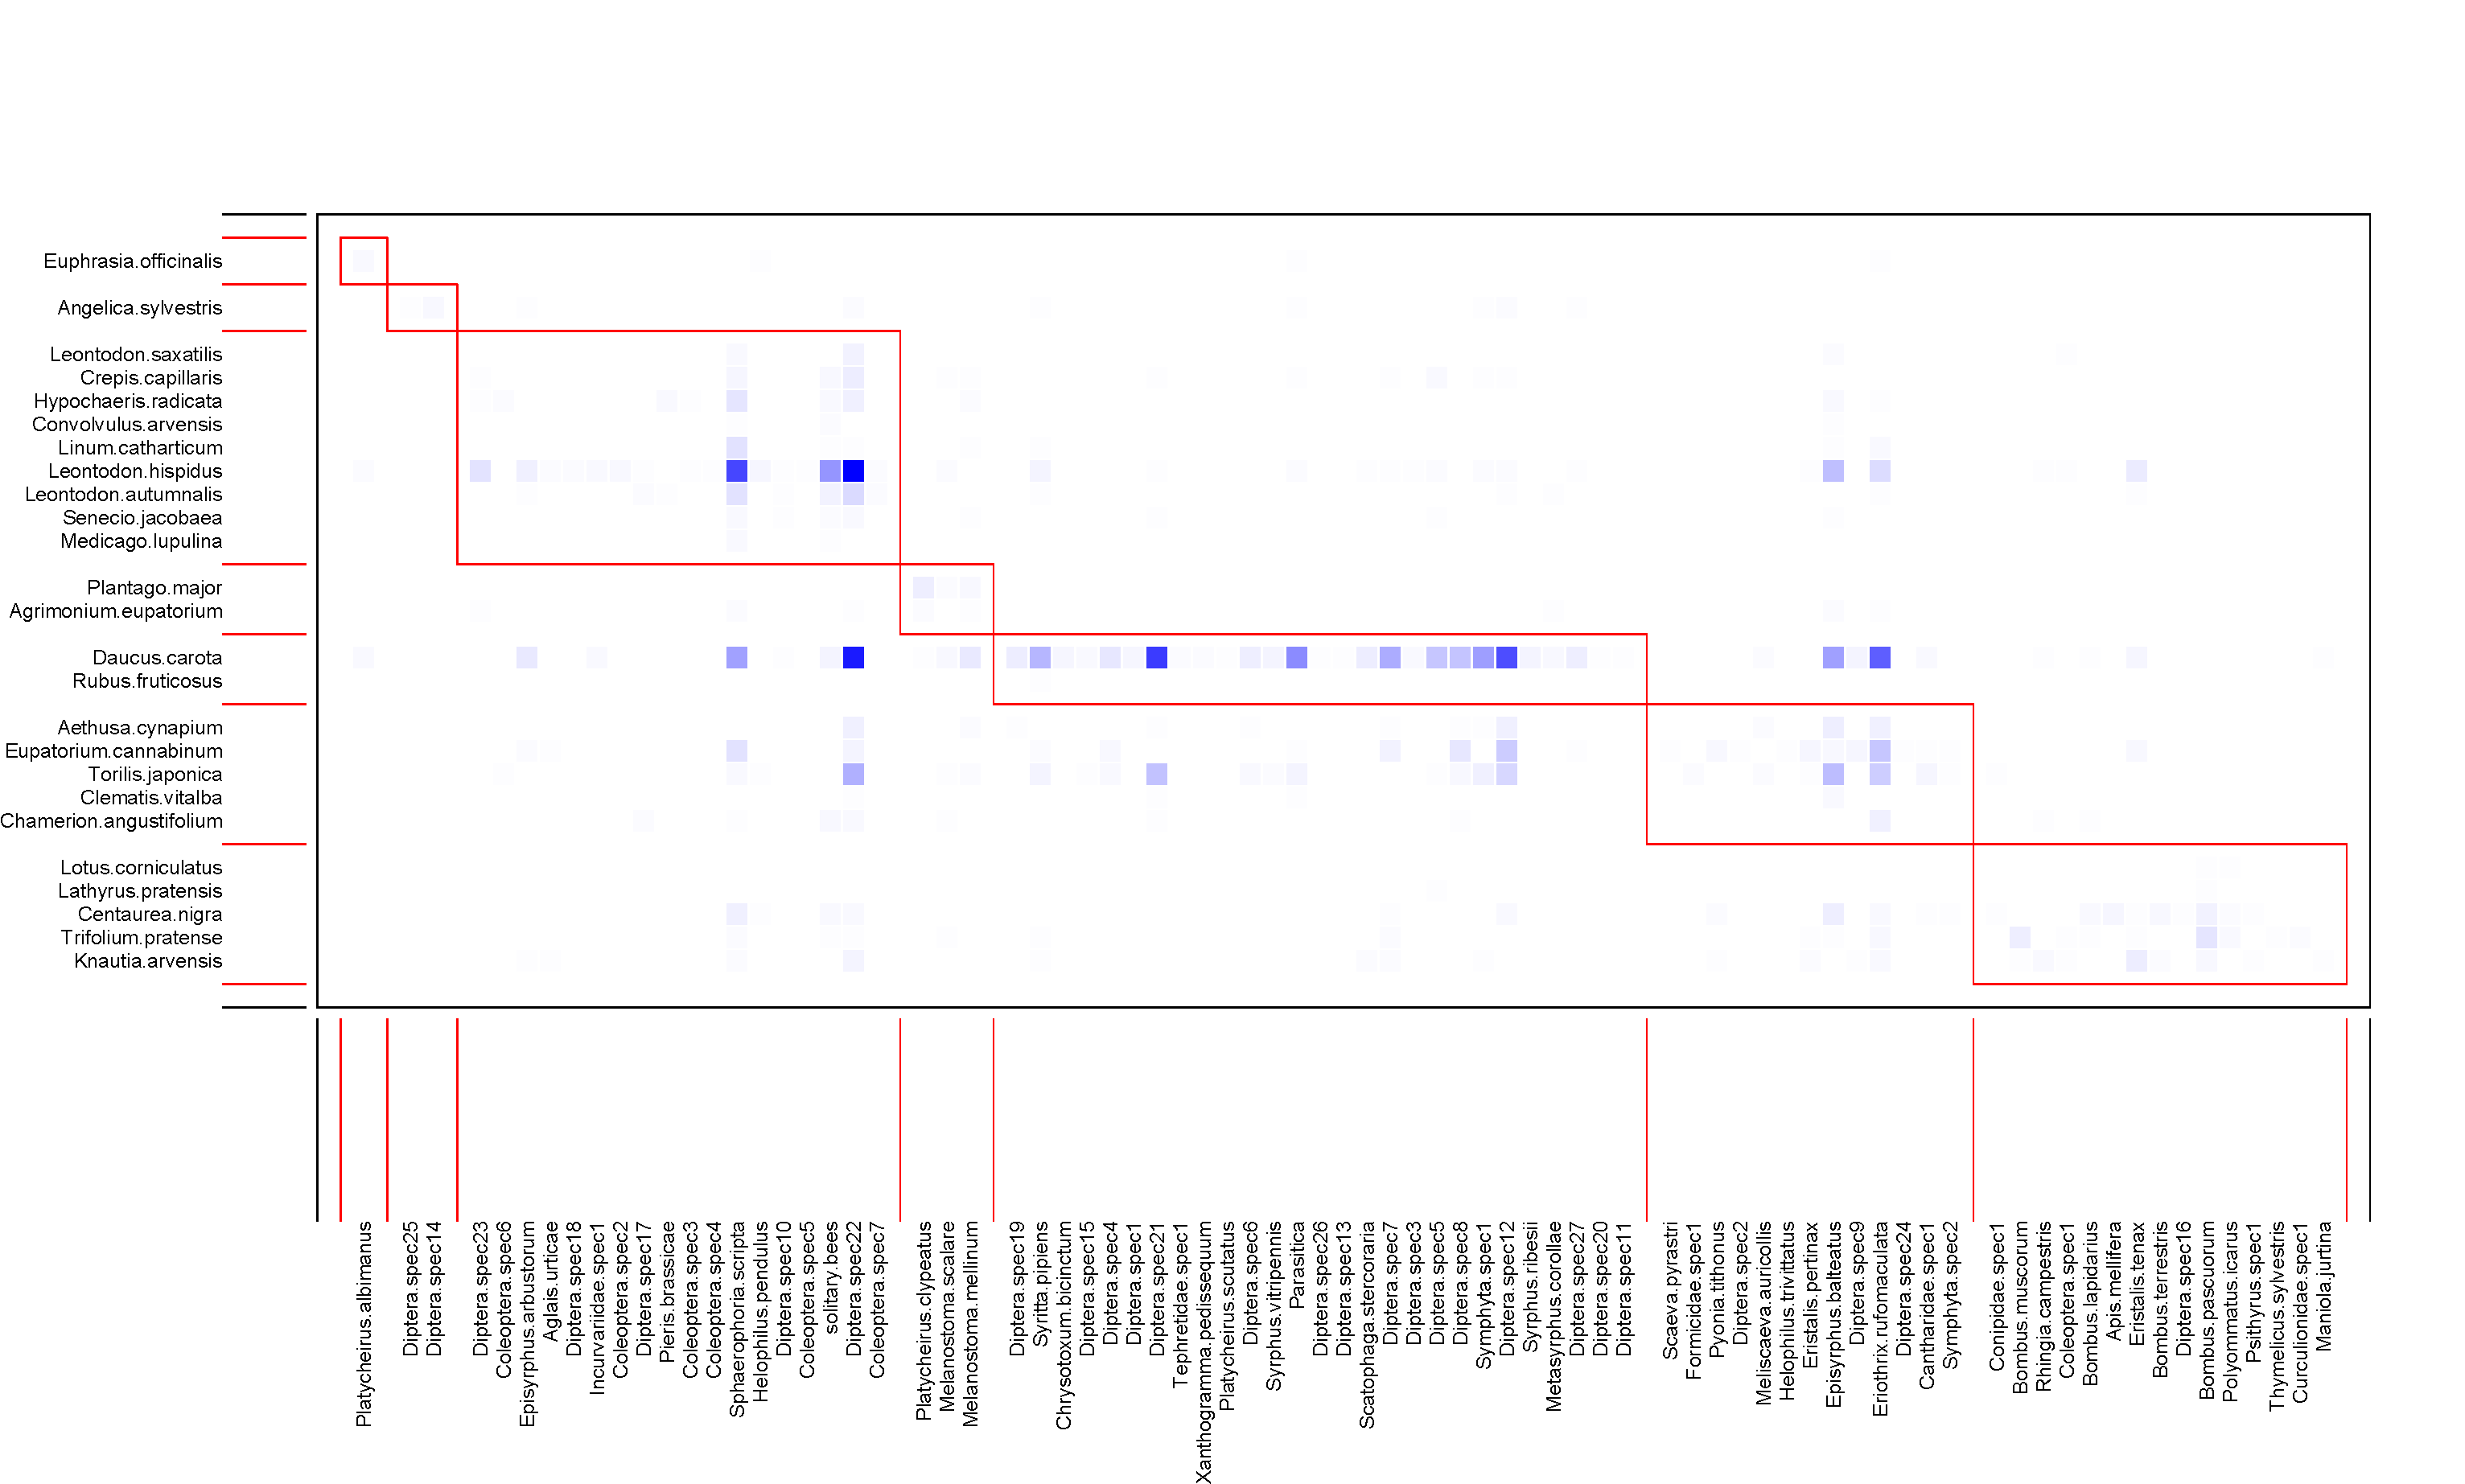
\includegraphics[width=\textwidth]{figures/memmott1999_modules_1E10}
	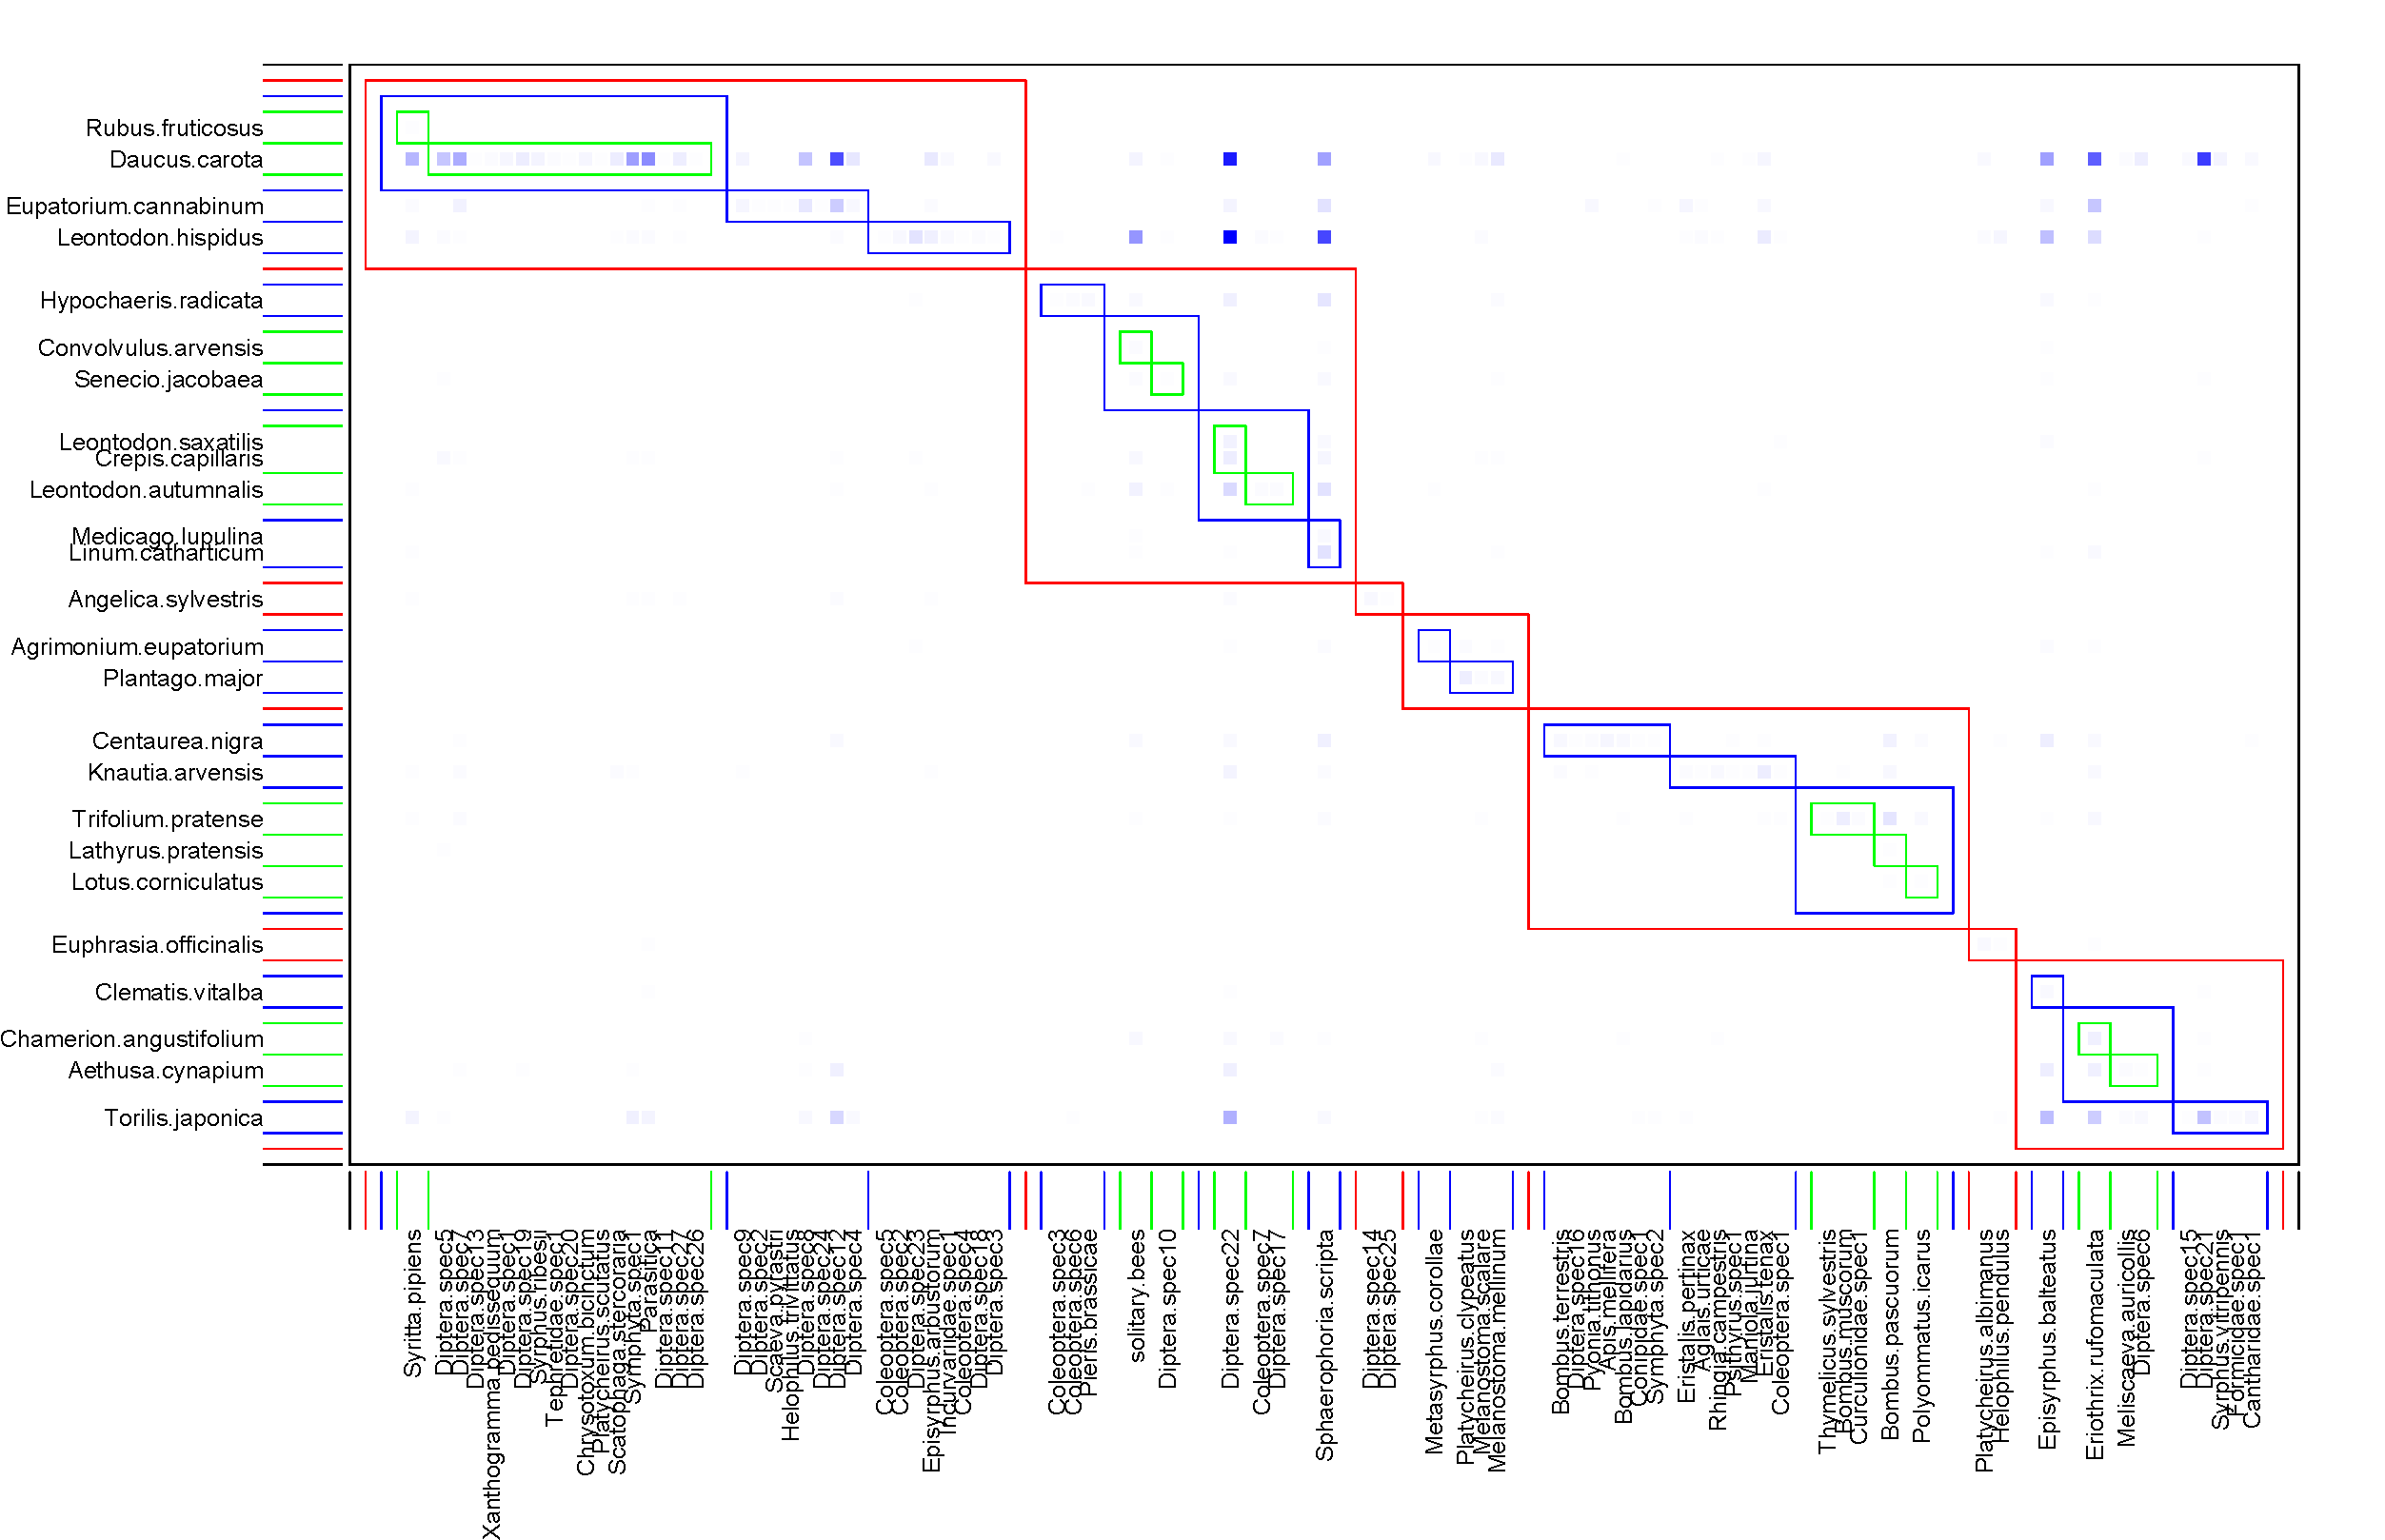
\includegraphics[width=0.8\textwidth]{figures/memmott1999_nested_modules}
	\caption{Interaction matrix featuring nested modules for the data of Memmott (1999). %\emph{Top}: Modules identified by QuaBiMo (with \texttt{steps=1e10}, running for several hours; $Q=0.30$). 
	Darker squares indicate more observed interactions. Coloured boxes delineate the seven modules. (Note that results may vary between runs.) In the central module yellow Asteraceae feature heavily, while a possible ecological cause pattern for the other modules is less apparent. %\emph{Bottom}: Nested modules based on a recursive call of QuaBiMo. Module arrangement is slightly different from top, since the algorithm is stochastic.
	}
\label{fig:memmottmodules}
\end{figure}

\begin{wrapfigure}{o}{0.3\textwidth}
	\vspace*{-.5cm}
	%\centering
	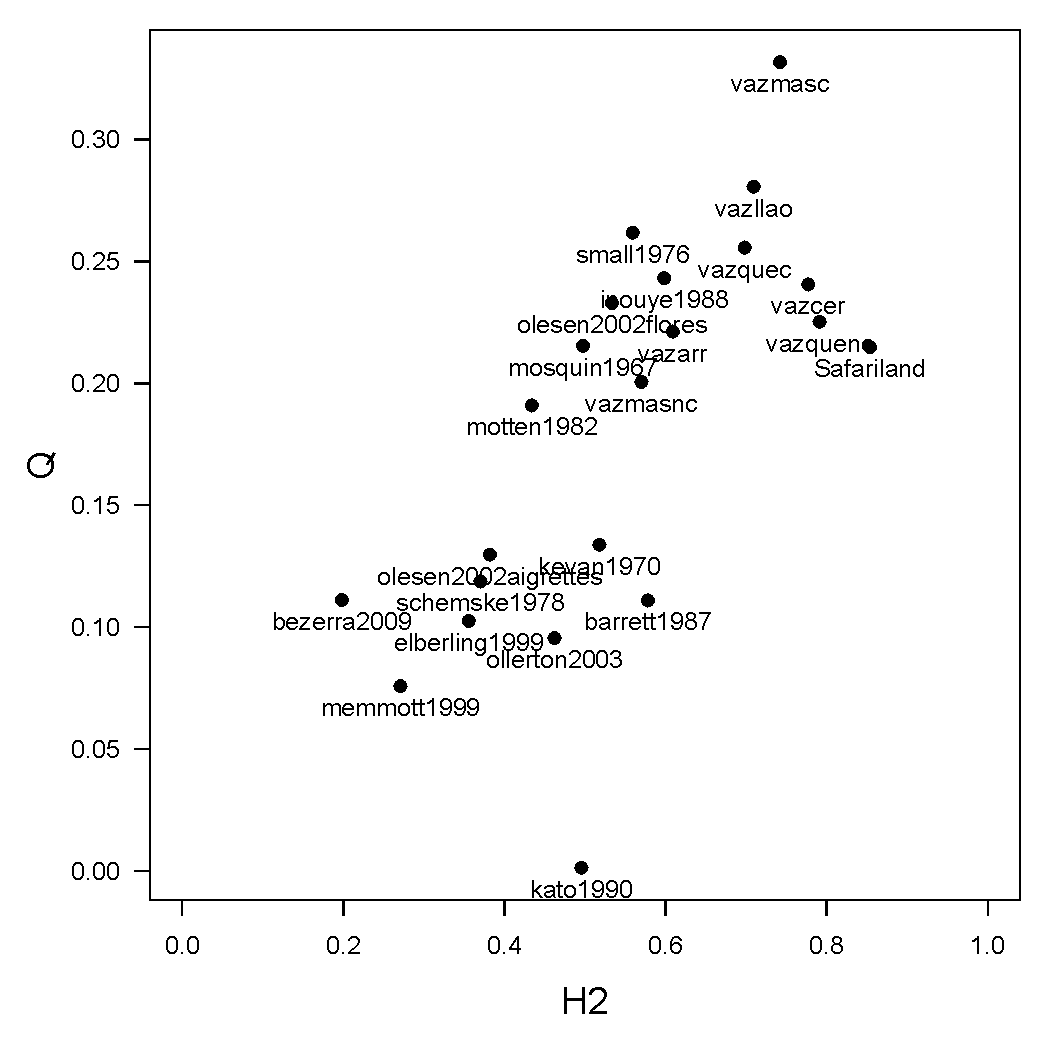
\includegraphics[width=0.3\textwidth]{figures/poll_mod_QvsH2}
	\caption{Modularity ($Q$) is highly correlated with specialisation $H_2'$ across $22$ pollination networks. Names refer to network data sets in \package{bipartite}.}
\label{fig:QvsH2}
\end{wrapfigure}
%
Modularity $Q$ is likely to be correlated with other network metric, as specialisation of module members is the prime reason for the existence of modules. Across the $22$ quantitative pollination networks of the NCEAS ``interaction webs'' data base,%\footnote{\url{http://www.nceas.ucsb.edu/interactionweb}}
 $Q$ was evidently highly positively correlated with complementary specialisation $H_2'$ (Fig.~\ref{fig:QvsH2}).
Ecologically, the correlation with specialisation makes good sense. Modules only exist because some species do not interact with some others, i.e. because they are specialised. An overall low degree of specialisation is equivalent to random interactions, which will yield no modules. % (unless as an artefact of low sampling intensity, which can be addressed using null models).

Furthermore, the absolute value of $Q$  is, like all network indices \citep{Dormann2009}, dependent on network size (i.e. the number of species) as well as the number of links and the total number of interactions observed \citep{Thebault2013}. We would thus recommend a null model comparison \citep{Vazquez2003a,Bluthgen2008,Dormann2009} to correct the observed value of $Q$ by null model expectation (e.g.~by standardising them to $z$-scores:
$z_{Q} = \frac{Q_{\text{observed}} - \overline{Q}_{\text{null}}}{\sigma_{Q_{\text{null}}}}$).
%
Modularity $Q$ is in itself not an index of an ecological feature. It is merely a measure of how well links and interactions can be separated into different modules. Large networks, with many species and links, allow for more combinations of species-in-modules, leading to higher values of $Q$, as \citet{Allesina2009a} pointed out for any grouping algorithm. %When some previous studies have not shown network size to be correlated with modularity, then that may indicate more the inadequacy of some algorithms than a deficit in those that do find a correlation.


\subsection{Using modularity to identifying species with important roles in the network}
\citet{Guimera2005} and \citet{Olesen2007} propose to compute standardised connection and participation values, called $c$ and $z$, for each species to describe their role in networks, where $c$ refers to the between-modules connectivity \citep[called ``participation coefficient'' $P$][]{Guimera2005} and $z$ refers to within-module degrees. Originally, both are computed based on the number of links, but a weighted version based on species strength is implemented, too. \citet{Guimera2005} suggest critical values (only for the binary approach) of $c$ and $z$ of $0.625$ and $2.5$, respectively. Species exceeding both of these values are called ``hubs'' because they link different modules, combining high between- with high within-module connectivity. 

In the case of the pollination network of Fig.~\ref{fig:memmottmodules}, $c$-values range between $0$ and $0.78$ (with $23$ of $79$ pollinators and $13$ of $25$ plant species exceeding the threshold of $0.625$); $z$-values range between $-1.21$ and $5.00$ (with two pollinators but no plant species exceeding the value of $2.5$: Fig.~\ref{fig:czvalues}). Put together, only the syrphid \emph{Syritta pipiens} (and hawkbit \emph{Leontodon hispidus} almost) exceeded both thresholds and would thus be called a ``hub species''. As can be seen in Fig.~\ref{fig:memmottmodules}, this syrphid is relatively rare but clearly not randomly distributed over the six modules, thus linking three highest-level modules. In contrast, \emph{Leontodon hispidus} is a common plant species, visited by many different pollinators, and it actually links almost all modules. 

%
\begin{figure}
\hfill
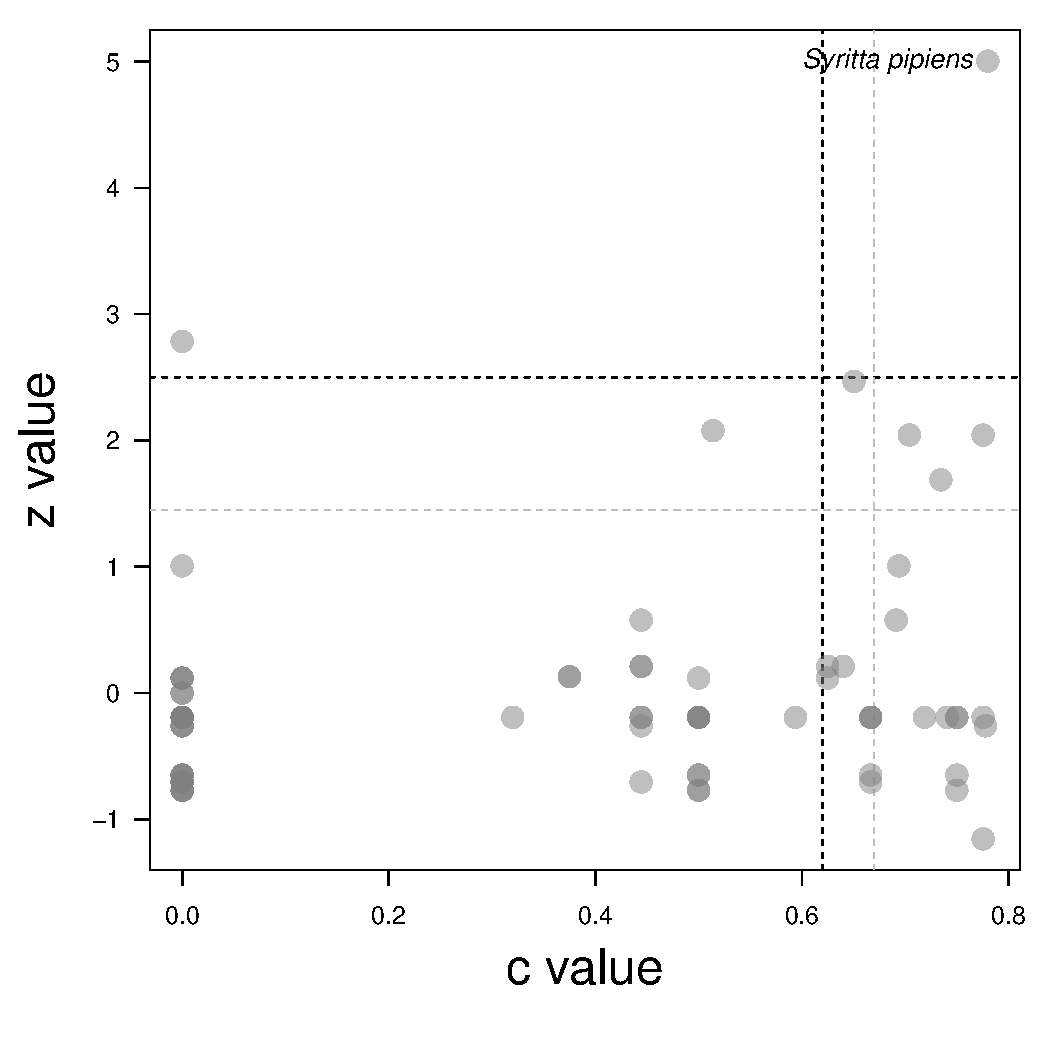
\includegraphics[width=0.48\textwidth]{figures/czvalues_memmott_pollinators}
\hfill
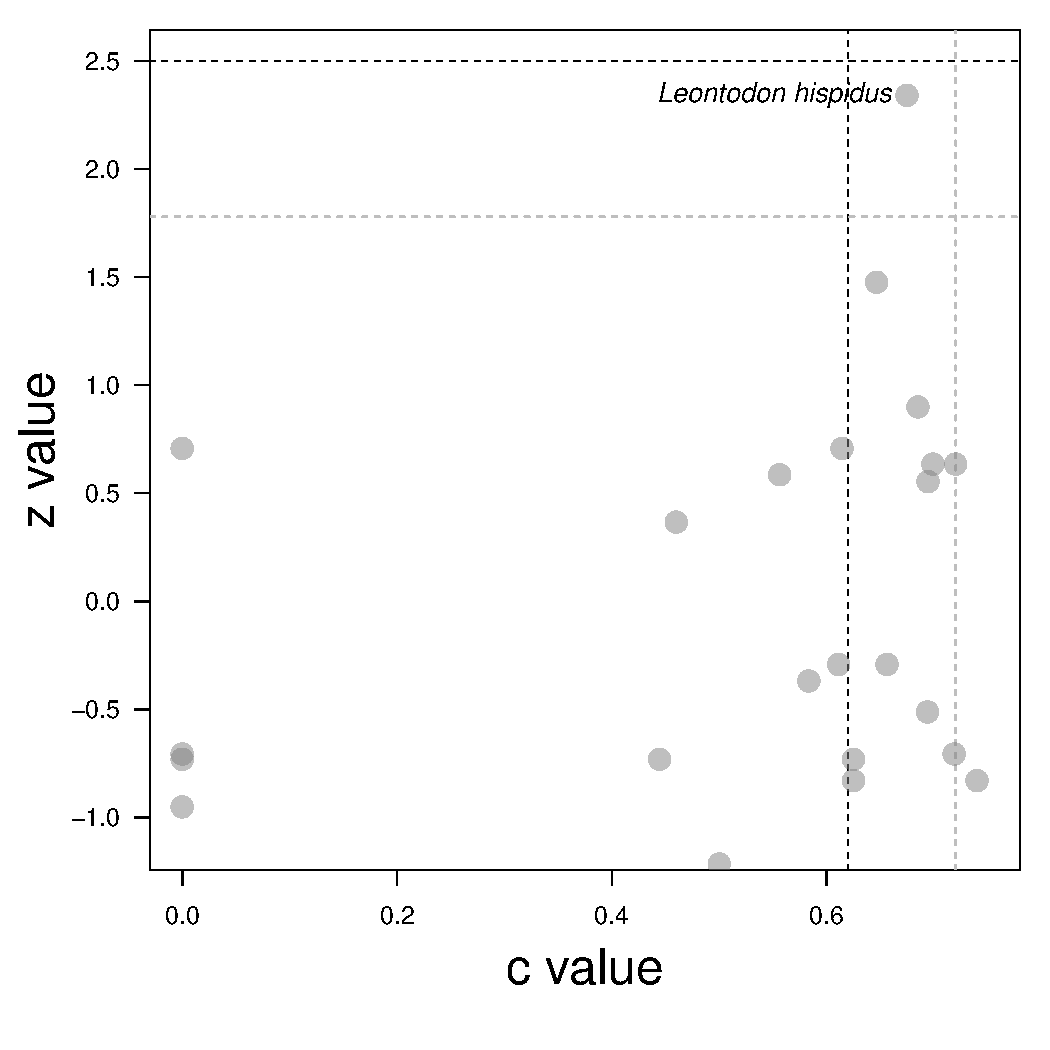
\includegraphics[width=0.48\textwidth]{figures/czvalues_memmott_plants}
\hfill
\caption{Connection ($c$) and participation ($z$) values for pollinators (left) and plants (right) in the network of Memmott (1999). Dashed black lines indicate critical values according to Olesen et al. (2007), those in grey $95$\% quantiles from $100$ null models (see text).}
\label{fig:czvalues}
\end{figure}
%
To objectively define this threshold one could run null models of the original network and employ $95$\% quantiles as critical $c$- and $z$-values. For the pollinators in the network of Fig.~\ref{fig:memmottmodules} these would be $0.67$ ($\pm 0.039$) and $1.45$ ($\pm 0.220$), respectively, based on $100$ null models (for plants: $c_\text{critical} = 0.72 \pm 0.036$ and $z_\text{critical} = 1.78 \pm 0.297$; Fig.~\ref{fig:czvalues} left). While for plant species this has little effect  (except for moving \emph{Leontodon hispidus} across the threshold), three more pollinators would become hub species (the common hoverfly \emph{Episyrphus balteatus}, the tachinid fly \emph{Eriothrix rufomaculata} and undetermined fly ``Diptera spec.22'').




\section*{Conclusions}%----------------------------------------------
The analysis of bipartite networks has seen a recent explosion of applications in ecology. The \proglang{R}-package \package{bipartite} aims at providing a user-friendly set of function to aid the visualisation and analysis of such networks. This vignette hopefully illustrated some of the  challenges and solutions to such analyses. The main take-home-message it aims to convey is that there are considerable interpretational strings attached, and that the analysis of bipartite networks is not as straightforward as one might have initially hoped.

\medskip
\noindent Feedback, improvements, corrections and additions are welcomed!







\bigskip

The Rnw source of this document is at \url{https://github.com/biometry/bipartite/bipartite/vignettes/Intro2bipartite.Rnw}.

%\backmatter % only if document type is book!
%\begin{fullwidth}
\setlength{\bibsep}{0cm}
\def\bibfont{\small}

\bibliographystyle{mee} %all show doi, url, isbn; haven't found out yet how to switch that off
\bibliography{bipartite}
%\end{fullwidth}

\printindex



\end{document}
